%===========================================================
% main.tex - 主控文件
%===========================================================
\documentclass[aspectratio=169, 12pt]{beamer}

% 导入配置文件
%===========================================================
% preamble.tex - Beamer 配置文件
%===========================================================

% 中文支持
\usepackage[UTF8]{ctex}

% 图形与表格
\usepackage{graphicx}
\usepackage{booktabs}

% 颜色与图形(必须在listings之前加载)
\usepackage{xcolor}
\usepackage{tikz}
\usetikzlibrary{shapes, arrows.meta, positioning}

% 数学公式
\usepackage{amsmath}
\usepackage{amssymb}

% 代码高亮
\usepackage{listings}

\lstset{
    language=Python,
    basicstyle=\small\ttfamily,
    keywordstyle=\color{blue},
    commentstyle=\color{green!60!black},
    stringstyle=\color{orange},
    breaklines=true,
    showstringspaces=false,
    keepspaces=true
}

% 超链接
\usepackage{hyperref}

%===========================================================
% 主题设置
%===========================================================
\usetheme{Madrid}
\usecolortheme{whale}
\usefonttheme{professionalfonts}

%===========================================================
% 课程信息
%===========================================================
\title[核心开发与调试]{第10周:核心开发与调试}
\subtitle{让系统真正跑起来}
\author{北京石油化工学院\textbackslash 人工智能研究院\textbackslash 王文通}
\institute{通选课}
\date{2025-2026 学年}

%===========================================================
% 自定义命令
%===========================================================
% 高亮命令
\newcommand{\highlight}[1]{\textcolor{red}{\textbf{#1}}}


% 学校信息(包含 logo 图片)
\institute{%
    \raisebox{-0.5cm}{\includegraphics[height=1.2cm]{../name.png}}\hspace{0.5cm}%
    \raisebox{-0.5cm}{\includegraphics[height=1.2cm]{../xiaohui.png}}\hspace{0.3cm}%
    \begin{minipage}{6cm}
        \centering
        \textbf{北京石油化工学院}\\
        \textit{人工智能研究院}
    \end{minipage}
}

\begin{document}

%===========================================================
% 标题页与目录
%===========================================================
\begin{frame}
    \titlepage
\end{frame}

\section*{课程概览}
\begin{frame}{课程概览}
    \begin{columns}
        \column{0.45\textwidth}
        \textbf{本周内容:}
        \begin{itemize}
            \item 项目回顾:已学模块快速串联
            \item 系统架构设计:分层架构与管道模式
            \item 模块接口设计规范
            \item 图像处理流水线实战
            \item AI辅助编程工具实战
            \item 团队协作与Git工作流
            \item 调试工具与项目框架
        \end{itemize}

        \column{0.55\textwidth}
        \textbf{Live Coding实战:}
        \begin{enumerate}
            \item 搭建项目框架(AI辅助)
            \item 实现图像处理流水线
            \item Git分支管理与协作
            \item 调试工具函数使用
            \item 团队分组与任务分配
        \end{enumerate}

        \vspace{0.3cm}
        \begin{block}{本周目标}
            搭建开发环境,完成70\%项目框架,开始模块开发
        \end{block}
    \end{columns}
\end{frame}

\begin{frame}{预备知识}
    \begin{block}{课前5分钟视频}
        \textbf{观看}: 软件架构基础、Python面向对象编程、Git基本操作
    \end{block}

    \vspace{0.3cm}

    \textbf{本周需要的前置知识:}
    \begin{columns}
        \column{0.5\textwidth}
        \begin{itemize}
            \item \textbf{软件工程基础}: 什么是架构、模块化思想
            \item \textbf{Python面向对象}: 类、继承、接口概念
            \item \textbf{Git基础}: add、commit、push操作
        \end{itemize}

        \column{0.5\textwidth}
        \begin{alertblock}{没有基础?}
        \begin{itemize}
            \item 课前观看预备知识视频
            \item 课堂上先观察架构图
            \item 小组讨论时向组员请教
            \item 课后查阅推荐资源
        \end{itemize}
        \end{alertblock}
    \end{columns}

    \vspace{0.3cm}

    \textbf{不同背景的学习建议:}
    \begin{table}
        \centering
        \small
        \begin{tabular}{lp{8cm}}
            \toprule
            \textbf{专业背景} & \textbf{学习建议} \\
            \midrule
            CS/EE专业 & 深入理解SOLID原则,尝试应用设计模式 \\
            数学/物理专业 & 关注架构的数学建模,理解模块依赖关系 \\
            其他专业 & 从架构图入手,理解模块分工,重点是团队协作 \\
            \bottomrule
        \end{tabular}
    \end{table}
\end{frame}

\begin{frame}{本周时间分配(135分钟 = 3学时)}
    \begin{columns}
        \column{0.5\textwidth}
        \textbf{第1学时(45分钟):}
        \begin{itemize}
            \item[00:00-00:05] 项目回顾(5min)
            \item[00:05-00:15] 架构设计概述(10min)
            \item[00:15-00:25] 分层架构与管道模式(10min)
            \item[00:25-00:40] Live Coding:搭建项目框架(15min)
            \item[00:40-00:45] 小组讨论:确定分工(5min)
        \end{itemize}

        \textbf{课间休息(10分钟):}
        \begin{itemize}
            \item[00:45-00:55] 休息与交流
        \end{itemize}

        \textbf{第2学时(40分钟):}
        \begin{itemize}
            \item[00:55-01:15] Live Coding:流水线实现(20min)
            \item[01:15-01:30] 实践环节:学生跟随编写(15min)
            \item[01:30-01:35] 小结与检查点(5min)
        \end{itemize}

        \column{0.5\textwidth}
        \textbf{第3学时(40分钟):}
        \begin{itemize}
            \item[01:35-01:50] AI辅助编程演示(15min)
            \item[01:50-02:05] 分组任务分配(15min)
            \item[02:05-02:10] 调试工具快速演示(5min)
            \item[02:10-02:15] 总结与作业(5min)
        \end{itemize}

        \vspace{0.3cm}
        \begin{block}{课后延伸}
        \begin{itemize}
            \item Git工作流:观看视频教程(课后)
            \item 案例分析:阅读材料(课后)
            \item 代码规范:参考文档(课后)
        \end{itemize}
        \end{block}

        \vspace{0.2cm}
        \begin{alertblock}{时间控制提示}
        Live Coding为核心(占50\%以上),理论讲解精简,重点在动手实践
        \end{alertblock}
    \end{columns}
\end{frame}

\begin{frame}{本周分组策略}
    \textbf{分组原则:}
    \begin{itemize}
        \item 每组3-4人
        \item 包含不同专业背景
        \item 设立组长和技术负责人
    \end{itemize}

    \vspace{0.3cm}

    \textbf{角色分工:}
    \begin{table}
        \centering
        \small
        \begin{tabular}{lp{6cm}l}
            \toprule
            \textbf{角色} & \textbf{职责} & \textbf{适合} \\
            \midrule
            组长 & 统筹协调、进度管理 & 组织能力强的 \\
            技术负责人 & 架构设计、核心算法 & CS/EE专业 \\
            模块开发A & 选择题+判断题实现 & 有编程基础的 \\
            模块开发B & 简答题+评分实现 & 有编程基础的 \\
            \bottomrule
        \end{tabular}
    \end{table}

    \vspace{0.3cm}

    \begin{block}{本周协作任务}
        搭建开发环境,开始模块开发(至少完成选择题框架)
    \end{block}
\end{frame}

%===========================================================
% 扩充版教学模块
%===========================================================
%===========================================================
% 00_background_expanded.tex - 背景知识铺垫(扩充版)
%===========================================================

\section{项目回顾:已学模块串联}

\begin{frame}{智能阅卷系统全景}
    \begin{center}
        \begin{tikzpicture}[scale=0.9, transform shape,
            box/.style={draw, rectangle, rounded corners, fill=blue!15, minimum width=2.5cm, minimum height=0.8cm, align=center},
            arrow/.style={->, thick, blue}]

            \node[box, fill=green!20] (input) at (0,0) {图像输入};
            \node[box, fill=blue!15] (preprocess) at (3,0) {预处理};
            \node[box, fill=blue!15] (layout) at (6,0) {版面分析};
            \node[box, fill=orange!15] (choice) at (9,0) {选择题};
            \node[box, fill=orange!15] (judge) at (12,0) {判断题};
            \node[box, fill=orange!15] (essay) at (15,0) {简答题};
            \node[box, fill=red!15] (output) at (18,0) {评分输出};

            \draw[arrow] (input) -- (preprocess);
            \draw[arrow] (preprocess) -- (layout);
            \draw[arrow] (layout) -- (choice);
            \draw[arrow] (layout) -- (judge);
            \draw[arrow] (layout) -- (essay);
            \draw[arrow] (choice) -- (output);
            \draw[arrow] (judge) -- (output);
            \draw[arrow] (essay) -- (output);
        \end{tikzpicture}
    \end{center}

    \textbf{本周任务:} 将所有模块整合,构建完整系统
\end{frame}

\begin{frame}{已学模块快速回顾}
    \begin{columns}
        \column{0.5\textwidth}
        \textbf{基础模块(第1-4周):}
        \begin{itemize}
            \item 图像基础:像素、通道、颜色空间
            \item 预处理:去噪、增强、二值化
            \item 几何变换:透视矫正
            \item 版面分析:边缘检测、轮廓提取
        \end{itemize}

        \column{0.5\textwidth}
        \textbf{识别模块(第5-8周):}
        \begin{itemize}
            \item 选择题:填涂检测、像素密度
            \item 判断题:符号识别、模板匹配
            \item 简答题:OCR识别、PaddleOCR
        \end{itemize}
    \end{columns}

    \vspace{0.3cm}

    \begin{alertblock}{本周目标}
        将散落的模块组装成完整的智能阅卷系统
    \end{alertblock}
\end{frame}

\begin{frame}{项目架构演进}
    \textbf{从"单文件"到"模块化":}

    \begin{center}
        \begin{tikzpicture}[scale=0.7, transform shape]
            % Before: Monolithic
            \node[draw, rectangle, fill=red!15, minimum width=3cm, minimum height=2cm, rounded corners] (mono) at (0,0) {
                \begin{small}
                main.py\\
                \hline
                load\_image()\\
                preprocess()\\
                detect()\\
                recognize()\\
                ...
                \end{small}
            };
            \node[below=0.2cm of mono] {\textbf{单文件(混乱)}};

            % Arrow
            \node at (4,0) {\Huge$\rightarrow$};

            % After: Modular
            \node[draw, rectangle, fill=green!15, minimum width=1.5cm, minimum height=1.5cm, rounded corners] (mod1) at (7,0) {preprocess\\.py};
            \node[draw, rectangle, fill=green!15, minimum width=1.5cm, minimum height=1.5cm, rounded corners] (mod2) at (9.5,0) {layout\\.py};
            \node[draw, rectangle, fill=green!15, minimum width=1.5cm, minimum height=1.5cm, rounded corners] (mod3) at (12,0) {recognition\\.py};

            \node[draw, rectangle, fill=blue!15, minimum width=4cm, minimum height=0.8cm, rounded corners] (main) at (9.5,-2) {main.py (框架)};

            \draw[-] (mod1) -- (main);
            \draw[-] (mod2) -- (main);
            \draw[-] (mod3) -- (main);
            \node[below=0.2cm of main] {\textbf{模块化(清晰)}};
        \end{tikzpicture}
    \end{center}
\end{frame}

\section{软件系统架构概述}

\begin{frame}{什么是软件架构?}
    \begin{definition}[软件架构]
        软件架构是系统的高级结构,包括软件元素、元素的外部可见属性,以及元素之间的关系。
    \end{definition}

    \vspace{0.3cm}

    \textbf{架构的核心要素:}
    \begin{itemize}
        \item \textbf{组件(Components)}:系统的功能单元,如模块、服务、类库
        \item \textbf{连接器(Connectors)}:组件之间的交互机制,如API调用、消息传递、事件
        \item \textbf{配置(Configuration)}:组件和连接器的拓扑结构,即系统的组织方式
        \item \textbf{约束(Constraints)}:设计和实现的规则,如技术选型、性能要求、安全规范
    \end{itemize}

    \vspace{0.3cm}

    \begin{alertblock}{架构 vs 设计}
        架构关注"系统由什么组成"和"它们如何交互";设计关注"如何实现每个组件"。
        架构是蓝图,设计是施工图。
    \end{alertblock}
\end{frame}

\begin{frame}{架构决策的层次}
    \begin{center}
        \begin{tikzpicture}[scale=0.85, transform shape,
            box/.style={draw, rectangle, rounded corners, fill=blue!15, minimum width=4cm, minimum height=0.8cm, align=center},
            arrow/.style={->, thick}]

            \node[box, fill=green!20] (business) at (0,0) {业务架构\\业务能力、流程};
            \node[box, fill=blue!20] (data) at (0,-1.2) {数据架构\\数据模型、存储};
            \node[box, fill=yellow!20] (app) at (0,-2.4) {应用架构\\模块划分、接口};
            \node[box, fill=red!20] (tech) at (0,-3.6) {技术架构\\技术选型、部署};

            \draw[arrow] (business) -- (data);
            \draw[arrow] (data) -- (app);
            \draw[arrow] (app) -- (tech);
        \end{tikzpicture}
    \end{center}

    \vspace{0.3cm}

    \textbf{各层次决策内容:}
    \begin{itemize}
        \item 业务架构:确定系统要解决什么问题,业务流程如何
        \item 数据架构:确定数据如何组织、存储、流转
        \item 应用架构:确定系统如何分解为可管理的模块
        \item 技术架构:确定使用什么技术栈,如何部署
    \end{itemize}
\end{frame}

\begin{frame}{架构设计的重要性}
    \begin{columns}
        \column{0.5\textwidth}
        \textbf{好的架构带来:}
        \begin{itemize}
            \item 易于理解和维护
            \item 便于团队协作
            \item 支持系统演化
            \item 降低技术风险
            \item 提高开发效率
            \item 支持快速迭代
        \end{itemize}

        \column{0.5\textwidth}
        \textbf{糟糕的架构导致:}
        \begin{itemize}
            \item 技术债务累积
            \item 修改牵一发而动全身
            \item 团队协作困难
            \item 系统难以扩展
            \item 维护成本高昂
            \item 新人难以入手
        \end{itemize}
    \end{columns}

    \vspace{0.5cm}

    \begin{block}{架构决策的影响}
        架构决策一旦做出,后期修改成本极高。前期投入时间设计架构是值得的。
        记住:修房子时改地基比建好后拆墙成本高得多。
    \end{block}
\end{frame}

\begin{frame}{架构设计原则:SOLID}
    \begin{table}
        \centering
        \small
        \begin{tabular}{clp{5.5cm}}
            \toprule
            \textbf{原则} & \textbf{名称} & \textbf{核心思想} \\
            \midrule
            S & 单一职责 & 一个类只负责一件事 \\
            O & 开闭原则 & 对扩展开放,对修改关闭 \\
            L & 里氏替换 & 子类可以替换父类 \\
            I & 接口隔离 & 客户端不应该依赖它不需要的接口 \\
            D & 依赖倒置 & 依赖抽象,而非具体实现 \\
            \bottomrule
        \end{tabular}
    \end{table}

    \vspace{0.3cm}

    \begin{exampleblock}{实际应用}
        \begin{itemize}
            \item SRP:图像预处理类只负责预处理,不负责识别
            \item OCP:新增识别算法时,不修改现有代码
            \item LSP:所有识别器可以互换使用
            \item ISP:按需定义小接口,而非大接口
            \item DIP:识别引擎依赖抽象接口,而非具体算法
        \end{itemize}
    \end{exampleblock}
\end{frame}

\begin{frame}{架构设计原则:KISS \& DRY}
    \begin{columns}
        \column{0.5\textwidth}
        \begin{block}{KISS原则}
            \textbf{K}eep \textbf{I}t \textbf{S}hort and \textbf{S}imple

            \vspace{0.3cm}
            \begin{itemize}
                \item 简单优于复杂
                \item 避免过度设计
                \item 选择最直接的解决方案
                \item 代码应易于理解
                \item 警惕"聪明的"代码
            \end{itemize}
        \end{block}

        \column{0.5\textwidth}
        \begin{block}{DRY原则}
            \textbf{D}on't \textbf{R}epeat \textbf{Y}ourself

            \vspace{0.3cm}
            \begin{itemize}
                \item 消除重复代码
                \item 单一事实来源
                \item 变化只需修改一处
                \item 提高可维护性
                \item 抽象重复逻辑
            \end{itemize}
        \end{block}
    \end{columns}

    \vspace{0.5cm}

    \begin{center}
        \textbf{简单是终极的复杂 —— 达芬奇}
    \end{center}
\end{frame}

\begin{frame}{架构风格分类}
    \begin{table}
        \centering
        \small
        \begin{tabular}{p{2.5cm}p{4cm}p{5cm}}
            \toprule
            \textbf{架构风格} & \textbf{特点} & \textbf{适用场景} \\
            \midrule
            单体架构 & 所有功能在一个应用中 & 小型项目、快速原型 \\
            分层架构 & 按层次组织 & 企业应用、Web应用 \\
            微服务架构 & 服务拆分、独立部署 & 大型系统、团队协作 \\
            事件驱动 & 基于事件通信 & 实时系统、流处理 \\
            管道-过滤器 & 数据流处理 & 数据处理、编译器 \\
            \bottomrule
        \end{tabular}
    \end{table}

    \vspace{0.3cm}

    \begin{alertblock}{选择建议}
        没有最好的架构,只有最适合的架构。根据团队规模、项目复杂度、维护周期选择。
        对于我们的智能阅卷系统,建议采用分层+管道过滤器混合架构。
    \end{alertblock}
\end{frame}

\begin{frame}{架构风格:分层架构详解}
    \begin{center}
        \begin{tikzpicture}[scale=0.8, transform shape,
            box/.style={draw, rectangle, rounded corners, minimum width=3.5cm, minimum height=0.8cm, align=center}]
            \node[box, fill=blue!20] (ui) at (0,0) {表现层 (UI/API)};
            \node[box, fill=green!20] (biz) at (0,-1.3) {业务层 (Services)};
            \node[box, fill=yellow!20] (domain) at (0,-2.6) {领域层 (Domain)};
            \node[box, fill=red!20] (data) at (0,-3.9) {数据层 (Repository)};

            \draw[->, thick] (ui) -- (biz);
            \draw[->, thick] (biz) -- (domain);
            \draw[->, thick] (domain) -- (data);
            \draw[->, thick] (data) -- (domain);
            \draw[->, thick] (domain) -- (biz);
            \draw[->, thick] (biz) -- (ui);
        \end{tikzpicture}
    \end{center}

    \textbf{分层架构的优点:}
    \begin{itemize}
        \item 关注点分离,职责清晰
        \item 易于测试(每层可独立测试)
        \item 便于维护(修改一层不影响其他层)
        \item 支持替换(如更换数据库)
        \item 新人容易理解代码结构
    \end{itemize}
\end{frame}

\begin{frame}{架构风格:微服务架构}
    \begin{center}
        \begin{tikzpicture}[scale=0.75, transform shape,
            box/.style={draw, rectangle, rounded corners, minimum width=2cm, minimum height=0.8cm, align=center},
            arrow/.style={->, thick}]

            \node[box, fill=blue!15] (gateway) at (0,0) {API网关};
            \node[box, fill=green!15] (upload) at (-4,-2) {上传服务};
            \node[box, fill=green!15] (process) at (-1.5,-2) {预处理服务};
            \node[box, fill=green!15] (recognize) at (1.5,-2) {识别服务};
            \node[box, fill=green!15] (grade) at (4,-2) {评分服务};
            \node[box, fill=red!15] (db1) at (-4,-4) {DB};
            \node[box, fill=red!15] (db2) at (1.5,-4) {DB};
            \node[box, fill=red!15] (db3) at (4,-4) {DB};

            \draw[arrow] (gateway) -- (upload);
            \draw[arrow] (gateway) -- (process);
            \draw[arrow] (gateway) -- (recognize);
            \draw[arrow] (gateway) -- (grade);
            \draw[arrow] (upload) -- (db1);
            \draw[arrow] (recognize) -- (db2);
            \draw[arrow] (grade) -- (db3);
        \end{tikzpicture}
    \end{center}

    \textbf{微服务特点:}
    \begin{itemize}
        \item 每个服务独立部署、独立扩展
        \item 服务间通过API通信
        \item 每个服务可以有独立的数据库
        \item 技术选型可以不同
        \item 适合大型团队
    \end{itemize}

    \begin{alertblock}{注意}
        微服务不是银词。对于小团队,单体应用往往更高效。
        阅卷系统当前阶段建议用单体,分层清晰即可。
    \end{alertblock}
\end{frame}

\begin{frame}{架构风格:管道-过滤器架构}
    \begin{center}
        \begin{tikzpicture}[scale=0.75, transform shape,
            box/.style={draw, rectangle, rounded corners, fill=blue!15, minimum width=1.8cm, minimum height=1cm}]

            \node[box, fill=green!20] (source) at (0,0) {数据源};
            \node[box] (f1) at (2.5,0) {Filter 1};
            \node[box] (f2) at (5,0) {Filter 2};
            \node[box] (f3) at (7.5,0) {Filter 3};
            \node[box, fill=red!20] (sink) at (10,0) {数据汇};

            \draw[->, thick] (source) -- (f1) node[midway, above] {Pipe};
            \draw[->, thick] (f1) -- (f2) node[midway, above] {Pipe};
            \draw[->, thick] (f2) -- (f3) node[midway, above] {Pipe};
            \draw[->, thick] (f3) -- (sink);
        \end{tikzpicture}
    \end{center}

    \textbf{管道-过滤器特点:}
    \begin{itemize}
        \item 数据流驱动,单向流动
        \item 每个过滤器独立,可复用
        \item 易于扩展,新增过滤器
        \item 支持并行处理
        \item 天然适合图像处理流程
    \end{itemize}

    \textbf{我们的应用:}
    \begin{center}
        图像输入 $\to$ 去噪 $\to$ 增强 $\to$ 二值化 $\to$ 矫正 $\to$ 版面分析
    \end{center}
\end{frame}

\begin{frame}{架构风格:事件驱动架构}
    \begin{definition}[事件驱动架构]
        系统组件通过发布和订阅事件进行通信,实现松耦合的交互模式。
    \end{definition}

    \begin{center}
        \begin{tikzpicture}[scale=0.75, transform shape,
            box/.style={draw, rectangle, rounded corners, fill=blue!15, minimum width=2cm, minimum height=0.8cm, align=center}]

            \node[box, fill=green!20] (pub) at (0,0) {事件发布者};
            \node[box, fill=yellow!20] (bus) at (4,0) {事件总线};
            \node[box, fill=red!15] (sub1) at (7,-1.5) {订阅者1};
            \node[box, fill=red!15] (sub2) at (7,0) {订阅者2};
            \node[box, fill=red!15] (sub3) at (7,1.5) {订阅者3};

            \draw[->, thick] (pub) -- (bus) node[midway, above] {事件};
            \draw[->, thick] (bus) -- (sub1);
            \draw[->, thick] (bus) -- (sub2);
            \draw[->, thick] (bus) -- (sub3);
        \end{tikzpicture}
    \end{center}

    \textbf{适用场景:}
    \begin{itemize}
        \item 异步处理:如图像处理完成后通知评分模块
        \item 解耦系统:发布者和订阅者互不感知
        \item 多端同步:Web、移动端同时接收更新
        \item 审计追踪:所有事件可记录
    \end{itemize}
\end{frame}

\section{智能阅卷系统架构分析}

\begin{frame}{智能阅卷系统的业务场景}
    \begin{columns}
        \column{0.5\textwidth}
        \textbf{主要用户:}
        \begin{itemize}
            \item 教师:上传试卷、查看结果、导出成绩
            \item 学生:查看成绩、提交复查申请
            \item 管理员:系统管理、用户管理
        \end{itemize}

        \column{0.5\textwidth}
        \textbf{用户痛点:}
        \begin{itemize}
            \item 人工阅卷耗时费力
            \item 容易出现人工错误
            \item 统计报表生成麻烦
            \item 无法追溯阅卷过程
        \end{itemize}
    \end{columns}

    \begin{center}
        \begin{tikzpicture}[scale=0.7, transform shape,
            box/.style={draw, rectangle, rounded corners, fill=blue!10, minimum width=2cm, minimum height=0.8cm}]
            \node[box] (upload) at (0,0) {上传试卷};
            \node[box] (process) at (0,-1.2) {图像处理};
            \node[box] (analyze) at (0,-2.4) {版面分析};
            \node[box] (recog) at (0,-3.6) {内容识别};
            \node[box] (grade) at (0,-4.8) {自动评分};
            \node[box] (export) at (0,-6) {结果导出};

            \draw[->, thick] (upload) -- (process);
            \draw[->, thick] (process) -- (analyze);
            \draw[->, thick] (analyze) -- (recog);
            \draw[->, thick] (recog) -- (grade);
            \draw[->, thick] (grade) -- (export);
        \end{tikzpicture}
    \end{center}
\end{frame}

\begin{frame}{系统功能需求分析}
    \begin{columns}
        \column{0.5\textwidth}
        \textbf{核心功能:}
        \begin{itemize}
            \item 图像导入与格式转换
            \item 图像预处理(去噪、矫正)
            \item 答题卡区域定位
            \item 选择题自动识别
            \item 判断题符号识别
            \item 简答题文字识别
            \item 答案比对与评分
            \item 成绩统计与导出
        \end{itemize}

        \column{0.5\textwidth}
        \textbf{辅助功能:}
        \begin{itemize}
            \item 标准答案管理
            \item 人工复核接口
            \item 识别结果校对
            \item 批量处理
            \item 历史记录查询
            \item 权限管理
            \item 日志记录
        \end{itemize}
    \end{columns}
\end{frame}

\begin{frame}{非功能性需求}
    \begin{table}
        \centering
        \small
        \begin{tabular}{lp{3cm}p{6cm}}
            \toprule
            \textbf{需求类型} & \textbf{具体要求} & \textbf{实现策略} \\
            \midrule
            性能 & 单张试卷<3秒 & 算法优化、并行处理、缓存 \\
            准确率 & 选择题>99\% & 多算法融合、人工复核机制 \\
            可扩展性 & 支持新题型 & 插件化架构、模块化设计 \\
            可用性 & 7x24小时 & 容错设计、异常恢复 \\
            安全性 & 数据加密 & 传输加密、访问控制 \\
            可维护性 & 易于升级 & 清晰文档、单元测试 \\
            可用性 & 简单易用 & 清晰UI、完善帮助 \\
            \bottomrule
        \end{tabular}
    \end{table}

    \begin{block}{性能要求详解}
        \begin{itemize}
            \item 图像预处理:<500ms/张
            \item 区域定位:<300ms/张
            \item 识别响应:<1.5s/题
            \item 评分汇总:<200ms
        \end{itemize}
    \end{block}
\end{frame}

\begin{frame}{典型智能阅卷系统架构案例}
    \begin{center}
        \begin{tikzpicture}[scale=0.7, transform shape,
            box/.style={draw, rectangle, rounded corners, minimum width=2.5cm, minimum height=0.8cm, align=center}]
            % 客户端层
            \node[box, fill=blue!15] (web) at (-3,0) {Web客户端};
            \node[box, fill=blue!15] (mobile) at (0,0) {移动端};
            \node[box, fill=blue!15] (desktop) at (3,0) {桌面端};

            % API网关层
            \node[box, fill=green!15] (gateway) at (0,-1.5) {API网关\\负载均衡};

            % 服务层
            \node[box, fill=yellow!15] (upload) at (-4,-3) {上传服务};
            \node[box, fill=yellow!15] (process) at (-1.5,-3) {处理服务};
            \node[box, fill=yellow!15] (recognize) at (1.5,-3) {识别服务};
            \node[box, fill=yellow!15] (grade) at (4,-3) {评分服务};

            % 数据层
            \node[box, fill=red!15] (storage) at (-2,-4.5) {文件存储};
            \node[box, fill=red!15] (db) at (2,-4.5) {数据库};

            % 连接线
            \draw[->] (web) -- (gateway);
            \draw[->] (mobile) -- (gateway);
            \draw[->] (desktop) -- (gateway);
            \draw[->] (gateway) -- (upload);
            \draw[->] (gateway) -- (process);
            \draw[->] (gateway) -- (recognize);
            \draw[->] (gateway) -- (grade);
            \draw[->] (upload) -- (storage);
            \draw[->] (process) -- (storage);
            \draw[->] (recognize) -- (db);
            \draw[->] (grade) -- (db);
        \end{tikzpicture}
    \end{center}

    \vspace{0.3cm}
    \small 这是一个典型的分层微服务架构,支持水平扩展和高可用。
\end{frame}

\begin{frame}{案例对比分析}
    \begin{table}
        \centering
        \small
        \begin{tabular}{p{3cm}p{3cm}p{3.5cm}p{3cm}}
            \toprule
            \textbf{维度} & \textbf{小型系统} & \textbf{中型系统} & \textbf{大型系统} \\
            \midrule
            用户规模 & <1000 & 1000-10万 & 10万+ \\
            试卷量级 & 10份/天 & 1万份/天 & 100万份/天 \\
            架构风格 & 单体分层 & 微服务 & 分布式微服务 \\
            部署方式 & 单机部署 & 集群部署 & 云原生 \\
            识别算法 & 模板匹配 & 机器学习 & 深度学习 \\
            扩展性 & 低 & 中 & 高 \\
            \bottomrule
        \end{tabular}
    \end{table}

    \begin{alertblock}{选型建议}
        学生课程项目建议采用:单体分层架构 + 管道过滤器模式
        足够简单支撑当前需求,同时为未来扩展预留空间。
    \end{alertblock}
\end{frame}

\section{团队协作与分组开发}

\begin{frame}{敏捷开发方法论简介}
    \begin{definition}[敏捷开发]
        敏捷开发是一种以人为核心、迭代、循序渐进的软件开发方法。强调快速交付、持续改进和适应变化。
    \end{definition}

    \vspace{0.3cm}

    \textbf{敏捷宣言四大价值观:}
    \begin{enumerate}
        \item 个体和互动 高于 流程和工具
        \item 工作的软件 高于 详尽的文档
        \item 客户合作 高于 合同谈判
        \item 响应变化 高于 遵循计划
    \end{enumerate}

    \begin{block}{常用敏捷方法}
        \begin{itemize}
            \item \textbf{Scrum}:迭代开发、每日站会、冲刺计划
            \item \textbf{Kanban}:可视化工作流、限制在制品
            \item \textbf{XP}:极限编程、结对编程、测试驱动
        \end{itemize}
    \end{block}
\end{frame}

\begin{frame}{Scrum核心概念}
    \begin{center}
        \begin{tikzpicture}[scale=0.8, transform shape,
            box/.style={draw, rectangle, rounded corners, fill=blue!15, minimum width=2.5cm, minimum height=0.8cm, align=center}]

            \node[box, fill=green!20] (sprint) at (0,0) {Sprint (2-4周)};
            \node[box, fill=yellow!20] (planning) at (-3,-1.5) {Sprint计划会};
            \node[box, fill=yellow!20] (daily) at (0,-1.5) {每日站会};
            \node[box, fill=yellow!20] (review) at (3,-1.5) {评审会};
            \node[box, fill=red!20] (retro) at (0,-3) {回顾会};

            \draw[->, thick] (planning) -- (sprint);
            \draw[->, thick] (daily) -- (sprint);
            \draw[->, thick] (sprint) -- (review);
            \draw[->, thick] (review) -- (retro);
            \draw[->, thick] (retro) -- (planning) node[midway, left] {改进};
        \end{tikzpicture}
    \end{center}

    \textbf{Scrum角色:}
    \begin{itemize}
        \item Product Owner:产品负责人,定义需求优先级
        \item Scrum Master:流程专家,保证流程执行
        \item Team:开发团队,执行开发工作
    \end{itemize}

    \textbf{核心工件:}
    \begin{itemize}
        \item Product Backlog:产品待办列表
        \item Sprint Backlog:冲刺待办列表
        \item Increment:可交付的增量
    \end{itemize}
\end{frame}

\begin{frame}{Kanban可视化看板}
    \begin{center}
        \begin{tikzpicture}[scale=0.8, transform shape,
            col/.style={draw, rectangle, fill=gray!10, minimum width=3cm, minimum height=5cm, align=center},
            item/.style={anchor=west, font=\small}]

            \node[col] (todo) at (0,0) {
                \textbf{待办}\\[2mm]
                任务A\\
                任务B\\
                任务C
            };
            \node[col] (doing) at (4,0) {
                \textbf{进行中}\\[2mm]
                任务D
            };
            \node[col] (review) at (8,0) {
                \textbf{审查中}\\[2mm]
                任务E
            };
            \node[col] (done) at (12,0) {
                \textbf{已完成}\\[2mm]
                任务F\\
                任务G
            };

            \draw[->, thick, blue] (todo) -- (doing);
            \draw[->, thick, blue] (doing) -- (review);
            \draw[->, thick, blue] (review) -- (done);
        \end{tikzpicture}
    \end{center}

    \textbf{Kanban核心原则:}
    \begin{itemize}
        \item 可视化工作流
        \item 限制在制品(WIP Limit)
        \item 管理流动
        \item 持续改进
    \end{itemize}
\end{frame}

\begin{frame}{团队协作工具与流程}
    \begin{columns}
        \column{0.5\textwidth}
        \textbf{版本控制:}
        \begin{itemize}
            \item Git:分布式版本控制
            \item GitHub/GitLab:代码托管
            \item 分支策略:Git Flow / GitHub Flow
        \end{itemize}

        \column{0.5\textwidth}
        \textbf{项目管理:}
        \begin{itemize}
            \item Jira:企业级项目管理
            \item Trello:轻量级看板
            \item Notion:知识库+任务管理
        \end{itemize}
    \end{columns}

    \begin{columns}
        \column{0.5\textwidth}
        \textbf{沟通协作:}
        \begin{itemize}
            \item Slack/飞书:即时通讯
            \item 腾讯会议:视频会议
            \item 石墨文档:协作文档
        \end{itemize}

        \column{0.5\textwidth}
        \textbf{CI/CD工具:}
        \begin{itemize}
            \item GitHub Actions
            \item Jenkins
            \item GitLab CI
        \end{itemize}
    \end{columns}
\end{frame}

\begin{frame}{代码规范与版本控制}
    \textbf{Python代码规范(PEP 8):}
    \begin{itemize}
        \item 缩进:4个空格(不要用Tab)
        \item 行宽:每行不超过79字符
        \item 命名:模块小写、类驼峰、函数下划线
        \item 注释:文档字符串、行内注释
        \item 导入:每行一个导入、按标准库/第三方/本地分组
    \end{itemize}

    \begin{block}{Git提交规范}
        \begin{itemize}
            \item feat:新功能
            \item fix:修复bug
            \item docs:文档更新
            \item style:格式调整
            \item refactor:重构
            \item test:测试相关
            \item chore:构建/工具
        \end{itemize}
    \end{block}

    \textbf{Git工作流最佳实践:}
    \begin{enumerate}
        \item 功能开发从develop分支创建feature分支
        \item 提交信息清晰描述变更内容
        \item 代码审查(Code Review)后再合并
        \item 定期同步主分支,解决冲突尽早
        \item 标签标记重要版本
    \end{enumerate}
\end{frame}

\begin{frame}{团队沟通与冲突解决}
    \begin{block}{有效沟通原则}
        \begin{itemize}
            \item \textbf{清晰表达}:明确目标、背景、期望
            \item \textbf{主动同步}:定期汇报进度、暴露问题
            \item \textbf{倾听反馈}:理解他人观点、接受建议
            \item \textbf{文档留痕}:重要决策书面记录
        \end{itemize}
    \end{block}

    \textbf{常见冲突及解决:}
    \begin{table}
        \centering
        \small
        \begin{tabular}{p{3cm}p{7cm}}
            \toprule
            \textbf{冲突类型} & \textbf{解决策略} \\
            \midrule
            技术方案分歧 & 数据说话、原型验证、投票决定 \\
            任务分配不均 & 明确角色、轮换任务、互相帮助 \\
            代码风格不一致 & 统一规范、自动化检查、互相审查 \\
            进度延误 & 及时沟通、调整计划、寻求帮助 \\
            资源竞争 & 优先级排序、错峰使用 \\
            \bottomrule
        \end{tabular}
    \end{table}
\end{frame}
     % 背景知识铺垫(扩充版)
%===========================================================
% 07_patterns_extended.tex - 架构设计模式与SOLID(扩充版)
%===========================================================

\section{分层架构模式详解}

\begin{frame}{分层架构的概念与优势}
    \begin{definition}[分层架构]
        将系统按职责划分为多个层次,每层只与相邻层交互,上层依赖下层,下层不依赖上层。
    \end{definition}

    \begin{columns}
        \column{0.5\textwidth}
        \textbf{经典三层架构:}
        \begin{enumerate}
            \item \textbf{表现层}:UI、API接口、用户交互
            \item \textbf{业务层}:业务逻辑、业务规则
            \item \textbf{数据层}:数据访问、持久化存储
        \end{enumerate}

        \column{0.5\textwidth}
        \begin{center}
            \begin{tikzpicture}[scale=0.75, transform shape,
                box/.style={draw, rectangle, minimum width=3cm, minimum height=0.8cm, align=center}]
                \node[box, fill=blue!20] (ui) at (0,0) {表现层\\(Presentation)};
                \node[box, fill=green!20] (biz) at (0,-1.2) {业务层\\(Business)};
                \node[box, fill=red!20] (data) at (0,-2.4) {数据层\\(Data)};

                \draw[->, thick] (ui) -- (biz);
                \draw[->, thick] (biz) -- (data);
            \end{tikzpicture}
        \end{center}
    \end{columns}

    \textbf{分层架构的优势:}
    \begin{itemize}
        \item 关注点分离,职责清晰
        \item 易于测试(每层可独立测试)
        \item 便于维护(修改一层不影响其他层)
        \item 支持替换(如更换数据库)
    \end{itemize}
\end{frame}

\begin{frame}{分层架构的详细设计}
    \begin{center}
        \begin{tikzpicture}[scale=0.65, transform shape,
            box/.style={draw, rectangle, rounded corners, minimum width=2.5cm, minimum height=0.7cm, align=center}]

            \node[box, fill=blue!20] (api) at (0,0) {API层\\FastAPI/Flask};
            \node[box, fill=blue!20] (controller) at (0,-1) {Controller\\请求路由};
            \node[box, fill=green!20] (service) at (0,-2) {Service\\业务逻辑};
            \node[box, fill=green!20] (manager) at (0,-3) {Manager\\领域服务};
            \node[box, fill=yellow!20] (repository) at (0,-4) {Repository\\数据访问};
            \node[box, fill=red!20] (model) at (0,-5) {Model\\数据模型};

            \draw[->, thick] (api) -- (controller);
            \draw[->, thick] (controller) -- (service);
            \draw[->, thick] (service) -- (manager);
            \draw[->, thick] (manager) -- (repository);
            \draw[->, thick] (repository) -- (model);
        \end{tikzpicture}
    \end{center}

    \textbf{各层职责:}
    \begin{itemize}
        \item API/Controller:请求接收、参数校验、响应格式化
        \item Service:编排业务逻辑、事务管理
        \item Manager/Domain:核心业务规则
        \item Repository:数据CRUD操作
        \item Model:数据结构定义
    \end{itemize}
\end{frame}

\begin{frame}{层间通信与依赖管理}
    \textbf{依赖方向:}
    \begin{itemize}
        \item 依赖只能从上到下
        \item 上层调用下层接口
        \item 下层通过回调/事件通知上层
    \end{itemize}

    \textbf{依赖倒置原则(DIP)应用:}
    \begin{columns}
        \column{0.5\textwidth}
        \textbf{不好的做法:}
        \begin{itemize}
            \item 上层直接依赖下层实现
            \item 紧耦合
            \item 难以替换实现
        \end{itemize}
        \begin{center}
            \begin{tikzpicture}[scale=0.5, transform shape]
                \node[draw, rectangle] (high) at (0,1) {高层模块};
                \node[draw, rectangle] (low) at (0,-1) {低层模块};
                \draw[->, thick] (high) -- (low);
            \end{tikzpicture}
        \end{center}

        \column{0.5\textwidth}
        \textbf{好的做法:}
        \begin{itemize}
            \item 依赖抽象接口
            \item 低层实现接口
            \item 灵活替换
        \end{itemize}
        \begin{center}
            \begin{tikzpicture}[scale=0.5, transform shape]
                \node[draw, rectangle] (high) at (0,1) {高层模块};
                \node[draw, rectangle, dashed] (interface) at (0,0) {接口};
                \node[draw, rectangle] (low) at (0,-1) {低层模块};
                \draw[->, thick] (high) -- (interface);
                \draw[->, thick] (interface) -- (low);
            \end{tikzpicture}
        \end{center}
    \end{columns}
\end{frame}

\begin{frame}{分层架构的适用场景}
    \begin{table}
        \centering
        \small
        \begin{tabular}{p{3cm}p{8cm}}
            \toprule
            \textbf{适用场景} & \textbf{说明} \\
            \midrule
            企业应用 & ERP、CRM等业务系统,业务逻辑复杂 \\
            Web应用 & 前后端分离的Web系统 \\
            桌面应用 & 具有复杂业务逻辑的单机软件 \\
            移动端应用 & 具有本地业务处理的App \\
            课程项目 & 小型到中型项目,快速开发 \\
            \bottomrule
        \end{tabular}
    \end{table}

    \begin{alertblock}{不适用场景}
        \begin{itemize}
            \item 简单脚本工具(过度设计)
            \item 高性能计算(层间开销)
        \end{itemize}
    \end{alertblock}
\end{frame}

\section{管道-过滤器架构:图像处理专精}

\begin{frame}{为什么选择管道-过滤器?}
    \begin{definition}[管道-过滤器架构]
        数据从数据源流入,经过一系列处理组件(过滤器)转换,最终输出到数据汇。
    \end{definition}

    \textbf{非常适合图像处理的原因:}
    \begin{columns}
        \column{0.5\textwidth}
        \begin{itemize}
            \item 图像处理本质是"流式"转换
            \item 每个步骤独立可测试
            \item 易于组合和替换
            \item 天然支持并行处理
        \end{itemize}

        \column{0.5\textwidth}
        \textbf{智能阅卷流水线示例:}
        \begin{center}
            \begin{tikzpicture}[scale=0.6, transform shape,
                box/.style={draw, rectangle, rounded corners, fill=blue!15, minimum width=1.5cm, minimum height=0.7cm, align=center}]

                \node[box, fill=green!20] (source) at (0,0) {输入};
                \node[box] (f1) at (2.5,0) {去噪};
                \node[box] (f2) at (4.5,0) {二值化};
                \node[box] (f3) at (6.5,0) {版面分析};
                \node[box, fill=red!20] (sink) at (8.5,0) {识别};

                \draw[->, thick] (source) -- (f1);
                \draw[->, thick] (f1) -- (f2);
                \draw[->, thick] (f2) -- (f3);
                \draw[->, thick] (f3) -- (sink);
            \end{tikzpicture}
        \end{center}
    \end{columns}
\end{frame}
        \end{tikzpicture}
    \end{center}

    \textbf{特点:}
    \begin{itemize}
        \item 数据流驱动,单向流动
        \item 过滤器独立,可复用
        \item 易于扩展,新增过滤器
        \item 支持并行处理
        \item 天然适合图像处理流程
    \end{itemize}
\end{frame}

\begin{frame}{过滤器组合与复用}
    \textbf{组合方式:}
    \begin{enumerate}
        \item \textbf{线性管道}:A → B → C
        \item \textbf{分支管道}:A → B/C → D
        \item \textbf{合并管道}:A/B → C
        \item \textbf{反馈管道}:输出反馈到输入
    \end{enumerate}

    \textbf{图像处理流水线示例:}
    \begin{center}
        \begin{tikzpicture}[scale=0.65, transform shape,
            box/.style={draw, rectangle, rounded corners, fill=green!15, minimum width=1.5cm, minimum height=0.8cm}]
            \node[box, fill=green!20] (in) at (0,0) {输入图像};
            \node[box] (denoise) at (2.5,0) {去噪};
            \node[box] (binary) at (5,0) {二值化};
            \node[box] (correct) at (7.5,0) {矫正};
            \node[box] (segment) at (10,0) {分割};
            \node[box, fill=red!20] (out) at (12.5,0) {输出图像};

            \draw[->, thick] (in) -- (denoise);
            \draw[->, thick] (denoise) -- (binary);
            \draw[->, thick] (binary) -- (correct);
            \draw[->, thick] (correct) -- (segment);
            \draw[->, thick] -- (out);
        \end{tikzpicture}
    \end{center}

    \textbf{复用策略:}
    \begin{itemize}
        \item 将常用过滤器组合封装为"宏过滤器"
        \item 提供预定义的流水线模板
        \item 支持通过配置切换不同过滤器组合
    \end{itemize}
\end{frame}

\section{SOLID原则详解}

\begin{frame}{单一职责原则(SRP)}
    \begin{definition}[单一职责原则]
        一个类应该只有一个引起它变化的原因。换句话说,一个类应该只负责一件事。
    \end{definition}

    \textbf{违反SRP的例子:}
    \begin{columns}
        \column{0.5\textwidth}
        \begin{center}
            \textbf{违反SRP}
        \end{center}
        \begin{center}
            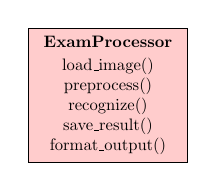
\begin{tikzpicture}[scale=0.6, transform shape]
                \node[draw, rectangle, fill=red!20, minimum width=3cm, minimum height=2cm] {
                    \begin{tabular}{c}
                        \textbf{ExamProcessor} \\[2pt]
                        load\_image() \\
                        preprocess() \\
                        recognize() \\
                        save\_result() \\
                        format\_output()
                    \end{tabular}
                };
            \end{tikzpicture}
        \end{center}

        \column{0.5\textwidth}
        \textbf{改进方案:}
        \begin{center}
            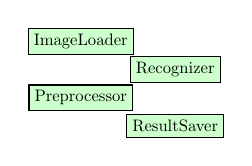
\begin{tikzpicture}[scale=0.6, transform shape]
                \node[draw, rectangle, fill=green!20] (loader) at (-1,0) {ImageLoader};
                \node[draw, rectangle, fill=green!20] (pre) at (-1,-1.2) {Preprocessor};
                \node[draw, rectangle, fill=green!20] (rec) at (1,-0.6) {Recognizer};
                \node[draw, rectangle, fill=green!20] (saver) at (1,-1.8) {ResultSaver};
            \end{tikzpicture}
        \end{center}
    \end{columns}

    \begin{itemize}
        \item SRP使得类更容易理解
        \item 修改只影响少量类
        \item 单元测试更容易编写
    \end{itemize}
\end{frame}

\begin{frame}{开闭原则(OCP)}
    \begin{definition}[开闭原则]
        软件实体应该对扩展开放,对修改关闭。
    \end{definition}

    \textbf{实现方式:}
    \begin{itemize}
        \item 抽象基类 + 具体实现
        \item 策略模式
        \item 依赖注入
        \item 插件架构
    \end{itemize}

    \begin{center}
        \begin{tikzpicture}[scale=0.7, transform shape,
            box/.style={draw, rectangle, minimum width=2.5cm, minimum height=0.7cm}]
            \node[draw, rectangle, dashed] (interface) at (0,0) {<<interface>>\\Recognizer};
            \node[box, fill=blue!15] (choice) at (-2,-1.5) {ChoiceRecognizer};
            \node[box, fill=blue!15] (judge) at (0,-1.5) {JudgeRecognizer};
            \node[box, fill=blue!15] (essay) at (2,-1.5) {EssayRecognizer};
            \node[box, fill=green!15, dashed] (new) at (4,-1.5) {NewRecognizer\\(扩展)};

            \draw[->, thick] (choice) -- (interface);
            \draw[->, thick] (judge) -- (interface);
            \draw[->, thick] (essay) -- (interface);
            \draw[->, thick, dashed] (new) -- (interface);
        \end{tikzpicture}
    \end{center}

    \textbf{OCP的好处:}
    \begin{itemize}
        \item 新功能通过添加新代码实现
        \item 现有代码不会被意外破坏
        \item 系统可维护性大大提高
    \end{itemize}
\end{frame}

\begin{frame}{里氏替换原则(LSP)}
    \begin{definition}[里氏替换原则]
        子类型必须能够替换其基类型,而程序的行为不会改变。
    \end{definition}

    \textbf{关键要求:}
    \begin{itemize}
        \item 子类不改变父类的前置条件(输入)
        \item 子类不强化父类的后置条件(输出)
        \item 子类保持父类的不变性
    \end{itemize}

    \textbf{正确示例:}
    \begin{center}
        \begin{tikzpicture}[scale=0.7, transform shape]
            \node[draw, rectangle, fill=blue!20] (parent) at (0,0) {
                \begin{tabular}{c}
                    \textbf{Recognizer} \\[2pt]
                    recognize(img) -> Result \\
                    preconditions: img不为None \\
                    postconditions: 返回Result对象
                \end{tabular}
            };

            \node[draw, rectangle, fill=green!20] (child) at (0,-2) {
                \begin{tabular}{c}
                    \textbf{OcrRecognizer (子类)} \\[2pt]
                    recognize(img) -> Result \\
                    接受相同输入,产生兼容输出
                \end{tabular}
            };

            \draw[->, thick] (child) -- (parent);
        \end{tikzpicture}
    \end{center}

    \begin{alertblock}{违反LSP的信号}
        \begin{itemize}
            \item 使用instanceof检查子类类型
            \item 需要知道具体子类才能调用
            \item 子类需要覆盖父类方法并抛出异常
        \end{itemize}
    \end{alertblock}
\end{frame}

\begin{frame}{接口隔离原则(ISP)}
    \begin{definition}[接口隔离原则]
        客户端不应该被迫依赖它不使用的方法。应该将大接口拆分为小接口。
    \end{definition}

    \textbf{不好的设计:}
    \begin{center}
        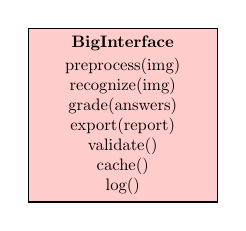
\begin{tikzpicture}[scale=0.6, transform shape]
            \node[draw, rectangle, fill=red!20, minimum width=4cm, minimum height=3cm] {
                \begin{tabular}{c}
                    \textbf{BigInterface} \\[2pt]
                    preprocess(img) \\
                    recognize(img) \\
                    grade(answers) \\
                    export(report) \\
                    validate() \\
                    cache() \\
                    log()
                \end{tabular}
            };
        \end{tikzpicture}
    \end{center}

    \textbf{改进设计:}
    \begin{center}
        \begin{tikzpicture}[scale=0.6, transform shape]
            \node[draw, rectangle, fill=green!15] (p) at (-2,0) {PreprocessorInterface};
            \node[draw, rectangle, fill=green!15] (r) at (0,0) {RecognizerInterface};
            \node[draw, rectangle, fill=green!15] (g) at (2,0) {GraderInterface};

            \node[draw, rectangle, fill=blue!15, minimum width=3cm, minimum height=1.5cm] (impl) at (0,-2) {
                ImageProcessor \\
                实现需要的接口
            };

            \draw[->, thick] (impl) -- (p);
            \draw[->, thick] (impl) -- (r);
            \draw[->, thick] (impl) -- (g);
        \end{tikzpicture}
    \end{center}
\end{frame}

\begin{frame}{依赖倒置原则(DIP)}
    \begin{definition}[依赖倒置原则]
        高层模块不应该依赖低层模块,两者都应该依赖抽象。抽象不应该依赖细节,细节应该依赖抽象。
    \end{definition}

    \textbf{示例对比:}
    \begin{columns}
        \column{0.5\textwidth}
        \textbf{传统方式(违反DIP):}
        \begin{center}
            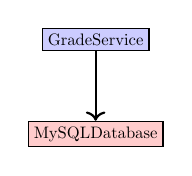
\begin{tikzpicture}[scale=0.6, transform shape]
                \node[draw, rectangle, fill=blue!20] (high) at (0,0) {GradeService};
                \node[draw, rectangle, fill=red!20] (low) at (0,-2) {MySQLDatabase};

                \draw[->, thick] (high) -- (low);
            \end{tikzpicture}
        \end{center}
        \begin{itemize}
            \item 高层依赖低层实现
            \item 更换数据库需要修改高层
            \item 难以测试
        \end{itemize}

        \column{0.5\textwidth}
        \textbf{改进方式(遵循DIP):}
        \begin{center}
            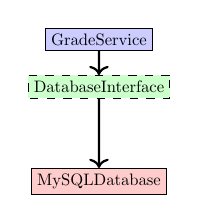
\begin{tikzpicture}[scale=0.6, transform shape]
                \node[draw, rectangle, fill=blue!20] (high) at (0,1) {GradeService};
                \node[draw, rectangle, dashed, fill=green!20] (interface) at (0,0) {DatabaseInterface};
                \node[draw, rectangle, fill=red!20] (low) at (0,-2) {MySQLDatabase};

                \draw[->, thick] (high) -- (interface);
                \draw[->, thick] (interface) -- (low);
            \end{tikzpicture}
        \end{center}
        \begin{itemize}
            \item 依赖抽象接口
            \item 可轻松替换实现
            \item 便于mock测试
        \end{itemize}
    \end{columns}
\end{frame}

\section{设计模式应用}

\begin{frame}{工厂模式}
    \begin{definition}[工厂模式]
        定义一个创建对象的接口,但让子类决定实例化哪个类。工厂方法让类将实例化推迟到子类。
    \end{definition}

    \begin{center}
        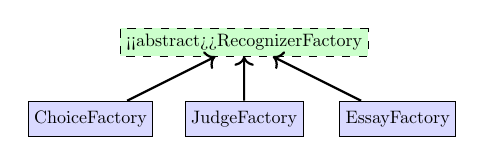
\begin{tikzpicture}[scale=0.65, transform shape,
            box/.style={draw, rectangle, minimum width=2cm, minimum height=0.7cm}]
            \node[draw, rectangle, dashed, fill=green!20] (factory) at (0,0) {<<abstract>>\\RecognizerFactory};
            \node[box, fill=blue!15] (choice) at (-3,-1.5) {ChoiceFactory};
            \node[box, fill=blue!15] (judge) at (0,-1.5) {JudgeFactory};
            \node[box, fill=blue!15] (essay) at (3,-1.5) {EssayFactory};

            \draw[->, thick] (choice) -- (factory);
            \draw[->, thick] (judge) -- (factory);
            \draw[->, thick] (essay) -- (factory);
        \end{tikzpicture}
    \end{center}

    \textbf{使用示例:}
    \begin{center}
        \begin{tikzpicture}[scale=0.7, transform shape]
            \node[draw, rectangle, fill=gray!10, minimum width=6cm, minimum height=2.5cm] {
                \begin{center}
                    \begin{tabular}{l}
                        \texttt{class RecognizerFactory:} \\
                        \texttt{    @staticmethod} \\
                        \texttt{    def create\_recognizer(type\_name):} \\
                        \texttt{        if type\_name == "choice":} \\
                        \texttt{            return ChoiceRecognizer()} \\
                        \texttt{        elif type\_name == "judge":} \\
                        \texttt{            return JudgeRecognizer()} \\
                        \texttt{        ...} \\
                        \\
                        \texttt{\# 使用} \\
                        \texttt{recognizer = RecognizerFactory.create\_recognizer("choice")}
                    \end{tabular}
                \end{center}
            };
        \end{tikzpicture}
    \end{center}
\end{frame}

\begin{frame}{策略模式}
    \begin{definition}[策略模式]
        定义一系列算法,将每个算法封装起来,使它们可以互相替换。策略让算法独立于使用它的客户端。
    \end{definition}

    \begin{center}
        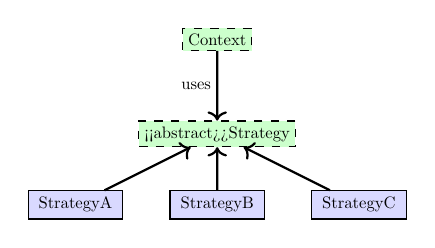
\begin{tikzpicture}[scale=0.6, transform shape,
            box/.style={draw, rectangle, minimum width=2cm, minimum height=0.6cm}]
            \node[draw, rectangle, dashed, fill=green!20] (context) at (0,1) {Context};
            \node[draw, rectangle, dashed, fill=green!20] (strategy) at (0,-1) {<<abstract>>\\Strategy};

            \node[box, fill=blue!15] (s1) at (-3,-2.5) {StrategyA};
            \node[box, fill=blue!15] (s2) at (0,-2.5) {StrategyB};
            \node[box, fill=blue!15] (s3) at (3,-2.5) {StrategyC};

            \draw[->, thick] (context) -- (strategy) node[midway, left] {uses};
            \draw[->, thick] (s1) -- (strategy);
            \draw[->, thick] (s2) -- (strategy);
            \draw[->, thick] (s3) -- (strategy);
        \end{tikzpicture}
    \end{center}

    \textbf{应用场景:}
    \begin{itemize}
        \item 多种识别算法切换
        \item 不同评分策略
        \item 多种输出格式
    \end{itemize}

    \textbf{优点:}
    \begin{itemize}
        \item 算法可以自由切换
        \item 避免使用条件语句
        \item 符合OCP原则
    \end{itemize}
\end{frame}

\begin{frame}{观察者模式}
    \begin{definition}[观察者模式]
        定义对象间的一种一对多依赖关系,当一个对象状态改变时,其所有依赖者都会收到通知并自动更新。
    \end{definition}

    \begin{center}
        \begin{tikzpicture}[scale=0.65, transform shape,
            box/.style={draw, rectangle, minimum width=1.8cm, minimum height=0.6cm}]
            \node[draw, rectangle, fill=yellow!20] (subject) at (0,0) {Subject\\主题};
            \node[box, fill=blue!15] (obs1) at (-3,-2) {Observer1};
            \node[box, fill=blue!15] (obs2) at (0,-2) {Observer2};
            \node[box, fill=blue!15] (obs3) at (3,-2) {Observer3};

            \draw[->, thick] (obs1) -- (subject);
            \draw[->, thick] (obs2) -- (subject);
            \draw[->, thick] (obs3) -- (subject);
            \draw[<->, thick] (subject) -- (obs1) node[midway, right] {notify};
            \draw[<->, thick] (subject) -- (obs2) node[midway, right] {notify};
            \draw[<->, thick] (subject) -- (obs3) node[midway, right] {notify};
        \end{tikzpicture}
    \end{center}

    \textbf{应用场景:}
    \begin{itemize}
        \item 识别完成通知评分模块
        \item 处理进度更新UI
        \item 日志记录事件
    \end{itemize}
\end{frame}

\begin{frame}{装饰器模式}
    \begin{definition}[装饰器模式]
        动态地给一个对象添加额外的职责,比生成子类更灵活。
    \end{definition}

    \begin{center}
        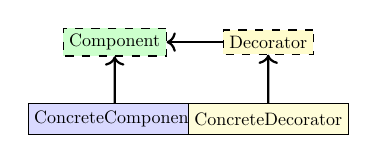
\begin{tikzpicture}[scale=0.65, transform shape,
            box/.style={draw, rectangle, minimum width=2cm, minimum height=0.6cm}]
            \node[draw, rectangle, dashed, fill=green!20] (component) at (0,0) {Component};
            \node[box, fill=blue!15] (concrete) at (0,-1.5) {ConcreteComponent};

            \node[draw, rectangle, dashed, fill=yellow!20] (decorator) at (3,0) {Decorator};
            \node[box, fill=yellow!15] (concreteD) at (3,-1.5) {ConcreteDecorator};

            \draw[->, thick] (concrete) -- (component);
            \draw[->, thick] (concreteD) -- (decorator);
            \draw[->, thick] (decorator) -- (component);
        \end{tikzpicture}
    \end{center}

    \textbf{使用示例:}
    \begin{center}
        \begin{tikzpicture}[scale=0.7, transform shape]
            \node[draw, rectangle, fill=gray!10, minimum width=6cm, minimum height=2.2cm] {
                \begin{center}
                    \begin{tabular}{l}
                        \texttt{class LoggingDecorator(RecognizerInterface):} \\
                        \texttt{    def \_\_init\_\_(self, recognizer):} \\
                        \texttt{        self.\_recognizer = recognizer} \\
                        \\
                        \texttt{    def recognize(self, image):} \\
                        \texttt{        print(f"开始识别")} \\
                        \texttt{        result = self.\_recognizer.recognize(image)} \\
                        \texttt{        print(f"识别完成: \{result\}")} \\
                        \texttt{        return result} \\
                        \\
                        \texttt{\# 使用:添加日志功能} \\
                        \texttt{logged\_rec = LoggingDecorator(basic\_rec)}
                    \end{tabular}
                \end{center}
            };
        \end{tikzpicture}
    \end{center}
\end{frame}

\begin{frame}{模板方法模式}
    \begin{definition}[模板方法模式]
        在抽象类中定义算法的骨架,将某些步骤的具体实现延迟到子类。
    \end{definition}

    \begin{center}
        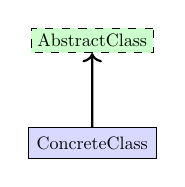
\begin{tikzpicture}[scale=0.65, transform shape,
            box/.style={draw, rectangle, minimum width=2.5cm, minimum height=0.6cm}]
            \node[draw, rectangle, dashed, fill=green!20] (abstract) at (0,0) {AbstractClass};
            \node[box, fill=blue!15] (concrete) at (0,-2) {ConcreteClass};

            \draw[->, thick] (concrete) -- (abstract);
        \end{tikzpicture}
    \end{center}

    \textbf{示例:图像处理流程}
    \begin{center}
        \begin{tikzpicture}[scale=0.7, transform shape]
            \node[draw, rectangle, fill=gray!10, minimum width=7cm, minimum height=2.5cm] {
                \begin{center}
                    \begin{tabular}{l}
                        \texttt{class ImageProcessor:} \\
                        \texttt{    def process(self, image):} \\
                        \texttt{        image = self.load(image)} \\
                        \texttt{        image = self.preprocess(image)} \\
                        \texttt{        image = self.analyze(image)} \\
                        \texttt{        return self.format\_result(image)} \\
                        \\
                        \texttt{    \# 子类实现具体步骤} \\
                        \texttt{    def preprocess(self, image): ...} \\
                        \texttt{    def analyze(self, image): ...}
                    \end{tabular}
                \end{center}
            };
        \end{tikzpicture}
    \end{center}
\end{frame}

\begin{frame}{设计模式总结对比}
    \begin{table}
        \centering
        \small
        \begin{tabular}{p{2cm}p{3cm}p{5cm}}
            \toprule
            \textbf{类型} & \textbf{模式} & \textbf{解决的问题} \\
            \midrule
            \textbf{创建型} & 工厂模式 & 对象创建逻辑复杂,类型需要运行时决定 \\
            & 单例模式 & 需要确保某个类只有一个实例 \\
            & 建造者模式 & 构建复杂对象,参数多,需分步骤构建 \\
            \midrule
            \textbf{结构型} & 适配器模式 & 接口不兼容,需要适配 \\
            & 装饰器模式 & 动态添加功能,不改变原有类 \\
            & 代理模式 & 控制访问,添加代理逻辑 \\
            \midrule
            \textbf{行为型} & 观察者模式 & 一对多通知,状态变化需广播 \\
            & 策略模式 & 算法可互换,需要运行时切换 \\
            & 模板方法 & 算法骨架固定,部分步骤可变 \\
            \bottomrule
        \end{tabular}
    \end{table}

    \begin{alertblock}{使用建议}
        不要为了使用模式而使用模式。只有当问题确实符合模式的应用场景时才使用。
        过度设计比设计不足更糟糕。
    \end{alertblock}
\end{frame}
        % 架构设计模式与SOLID(扩充版)
%===========================================================
% 08_pipeline_extended.tex - 图像处理流水线实战(扩充版)
%===========================================================

\section{流水线架构设计详解}

\begin{frame}{为什么选择管道-过滤器架构?}
    \begin{definition}[管道-过滤器架构]
        数据从数据源流入,经过一系列处理组件(过滤器)转换,最终输出到数据池。
    \end{definition}

    \begin{columns}
        \column{0.5\textwidth}
        \textbf{图像处理的特点:}
        \begin{itemize}
            \item 数据流明确:输入 $\to$ 处理 $\to$ 输出
            \item 步骤独立:去噪、增强、分割可独立工作
            \item 可组合:不同场景需要不同处理组合
            \item 可复用:过滤器可在多个流程中使用
        \end{itemize}

        \column{0.5\textwidth}
        \textbf{管道-过滤器的优势:}
        \begin{itemize}
            \item 高内聚:每个过滤器职责单一
            \item 低耦合:过滤器间通过标准接口连接
            \item 易扩展:添加新过滤器不影响现有
            \item 易测试:每个过滤器可独立测试
        \end{itemize}
    \end{columns}

    \begin{block}{适用场景}
        编译器、数据处理管道、音视频处理、图像处理、ETL流程
    \end{block}
\end{frame}

\begin{frame}{流水线整体架构}
    \begin{center}
        \begin{tikzpicture}[scale=0.7, transform shape,
            box/.style={draw, rectangle, rounded corners, fill=blue!15, minimum width=2.2cm, minimum height=0.9cm, align=center},
            pipe/.style={->, thick}]

            % 数据源
            \node[box, fill=green!20] (input) at (0,0) {原始图像};

            % 过滤器
            \node[box] (f1) at (2.8,0) {图像加载\\Loader};
            \node[box] (f2) at (5.6,0) {去噪\\Denoise};
            \node[box] (f3) at (8.4,0) {增强\\Enhance};
            \node[box] (f4) at (11.2,0) {二值化\\Binarize};
            \node[box] (f5) at (14,0) {矫正\\Correct};
            \node[box] (f6) at (16.8,0) {区域定位\\Locate};

            % 数据汇
            \node[box, fill=red!20] (output) at (19.6,0) {处理后图像};

            % 连接
            \draw[pipe] (input) -- (f1);
            \draw[pipe] (f1) -- (f2);
            \draw[pipe] (f2) -- (f3);
            \draw[pipe] (f3) -- (f4);
            \draw[pipe] (f4) -- (f5);
            \draw[pipe] (f5) -- (f6);
            \draw[pipe] (f6) -- (output);
        \end{tikzpicture}
    \end{center}

    \textbf{设计要点:}
    \begin{itemize}
        \item 每个过滤器职责单一
        \item 过滤器之间松耦合
        \item 支持动态组合
        \item 中间结果可追溯
    \end{itemize}
\end{frame}

\begin{frame}{数据流转设计}
    \begin{definition}[ImageData数据类]
        流水线中传递的数据封装,包含图像本身和处理过程中的元数据。
    \end{definition}

    \begin{block}{ImageData结构}
        \begin{itemize}
            \item \texttt{image: np.ndarray} - 原始/处理后图像
            \item \texttt{metadata: Dict} - 处理元数据(步骤、参数)
            \item \texttt{step\_name: str} - 当前处理步骤
            \item \texttt{confidence: float} - 处理置信度
        \end{itemize}
    \end{block}

    \textbf{元数据内容:}
    \begin{itemize}
        \item 处理步骤历史
        \item 每步参数配置
        \item 中间结果引用
        \item 时间戳记录
        \item 异常信息记录
    \end{itemize}
\end{frame}

\begin{frame}{过滤器接口设计}
    \begin{definition}[FilterInterface抽象基类]
        所有过滤器必须实现的接口规范。
    \end{definition}

    \begin{center}
        \begin{tikzpicture}[scale=0.7, transform shape]
            \node[draw, rectangle, fill=gray!10, minimum width=9cm, minimum height=5.5cm] {
                \centering
                \begin{tabular}{l}
                    \texttt{from abc import ABC, abstractmethod} \\
                    \texttt{from dataclasses import dataclass} \\
                    \texttt{from typing import Any, Dict} \\
                    \\
                    \texttt{@dataclass} \\
                    \texttt{class ImageData:} \\
                    \texttt{    """图像数据封装""" } \\
                    \texttt{    image: np.ndarray} \\
                    \texttt{    metadata: Dict[str, Any]} \\
                    \\
                    \texttt{class FilterInterface(ABC):} \\
                    \texttt{    """过滤器接口""" } \\
                    \\
                    \texttt{    @abstractmethod} \\
                    \texttt{    def process(self, data: ImageData) -> ImageData:} \\
                    \texttt{        """处理图像数据,返回处理后的数据""" } \\
                    \texttt{        pass} \\
                    \\
                    \texttt{    @abstractmethod} \\
                    \texttt{    def get\_name(self) -> str:} \\
                    \texttt{        """获取过滤器名称""" } \\
                    \texttt{        pass} \\
                    \\
                    \texttt{    def configure(self, params: Dict[str, Any]) -> None:} \\
                    \texttt{        """配置参数(可选)""" } \\
                    \texttt{        pass}
                \end{tabular}
            };
        \end{tikzpicture}
    \end{center}
\end{frame}

\section{过滤器实现详解}

\begin{frame}{去噪过滤器实现}
    \begin{center}
        \begin{tikzpicture}[scale=0.7, transform shape]
            \node[draw, rectangle, fill=gray!10, minimum width=9cm, minimum height=5cm] {
                \centering
                \begin{tabular}{l}
                    \texttt{class DenoiseFilter(FilterInterface):} \\
                    \texttt{    """去噪过滤器:高斯滤波""" } \\
                    \\
                    \texttt{    def \_\_init\_\_(self, kernel\_size=5):} \\
                    \texttt{        self.kernel\_size = kernel\_size} \\
                    \texttt{        self.name = "DenoiseFilter"} \\
                    \\
                    \texttt{    def get\_name(self) -> str:} \\
                    \texttt{        return self.name} \\
                    \\
                    \texttt{    def process(self, data: ImageData) -> ImageData:} \\
                    \texttt{        denoised = cv2.GaussianBlur(} \\
                    \texttt{            data.image,} \\
                    \texttt{            (self.kernel\_size, self.kernel\_size), 0} \\
                    \texttt{        )} \\
                    \texttt{        data.metadata['denoise\_applied'] = True} \\
                    \texttt{        data.metadata['kernel\_size'] = self.kernel\_size} \\
                    \texttt{        return ImageData(denoised, data.metadata)} \\
                    \\
                    \texttt{    def configure(self, params: Dict[str, Any]) -> None:} \\
                    \texttt{        self.kernel\_size = params.get('kernel\_size', 5)}
                \end{tabular}
            };
        \end{tikzpicture}
    \end{center}

    \begin{itemize}
        \item 参数可配置:核大小可调
        \item 元数据记录:标记已应用去噪
        \item 纯函数设计:输入输出明确
    \end{itemize}
\end{frame}

\begin{frame}{二值化过滤器实现}
    \begin{center}
        \begin{tikzpicture}[scale=0.7, transform shape]
            \node[draw, rectangle, fill=gray!10, minimum width=9cm, minimum height=5cm] {
                \centering
                \begin{tabular}{l}
                    \texttt{class BinarizeFilter(FilterInterface):} \\
                    \texttt{    """自适应二值化过滤器""" } \\
                    \\
                    \texttt{    def \_\_init\_\_(self, method='adaptive', block\_size=11):} \\
                    \texttt{        self.method = method} \\
                    \texttt{        self.block\_size = block\_size} \\
                    \texttt{        self.name = "BinarizeFilter"} \\
                    \\
                    \texttt{    def process(self, data: ImageData) -> ImageData:} \\
                    \texttt{        gray = cv2.cvtColor(data.image, cv2.COLOR\_BGR2GRAY)} \\
                    \\
                    \texttt{        if self.method == 'adaptive':} \\
                    \texttt{            binary = cv2.adaptiveThreshold(} \\
                    \texttt{                gray, 255, cv2.ADAPTIVE\_THRESH\_GAUSSIAN\_C,} \\
                    \texttt{                cv2.THRESH\_BINARY, self.block\_size, 2} \\
                    \texttt{            )} \\
                    \texttt{        else:} \\
                    \texttt{            \_, binary = cv2.threshold(gray, 127, 255, cv2.THRESH\_BINARY)} \\
                    \\
                    \texttt{        data.metadata['binarize\_method'] = self.method} \\
                    \texttt{        return ImageData(binary, data.metadata)}
                \end{tabular}
            };
        \end{tikzpicture}
    \end{center}
\end{frame}

\begin{frame}{透视矫正过滤器实现}
    \begin{center}
        \begin{tikzpicture}[scale=0.7, transform shape]
            \node[draw, rectangle, fill=gray!10, minimum width=9cm, minimum height=5cm] {
                \centering
                \begin{tabular}{l}
                    \texttt{class PerspectiveCorrectionFilter(FilterInterface):} \\
                    \texttt{    """透视矫正过滤器""" } \\
                    \\
                    \texttt{    def \_\_init\_\_(self, target\_points=None):} \\
                    \texttt{        self.target\_points = target\_points} \\
                    \texttt{        self.name = "PerspectiveCorrectionFilter"} \\
                    \\
                    \texttt{    def process(self, data: ImageData) -> ImageData:} \\
                    \texttt{        \# 从元数据获取角点} \\
                    \texttt{        corners = data.metadata.get('corners')} \\
                        \texttt{        if corners is None:} \\
                        \texttt{            return data  \# 无需矫正} \\
                        \\
                        \texttt{        \# 计算透视变换矩阵} \\
                        \texttt{        h, w = data.image.shape[:2]} \\
                        \texttt{        target = np.float32([[0, 0], [w, 0], [w, h], [0, h]])} \\
                        \texttt{        matrix = cv2.getPerspectiveTransform(corners, target)} \\
                        \\
                        \texttt{        \# 应用变换} \\
                        \texttt{        corrected = cv2.warpPerspective(data.image, matrix, (w, h))} \\
                        \texttt{        return ImageData(corrected, data.metadata)}
                    \end{tabular}
            };
        \end{tikzpicture}
    \end{center}
\end{frame}

\begin{frame}{区域定位过滤器}
    \begin{center}
        \begin{tikzpicture}[scale=0.7, transform shape]
            \node[draw, rectangle, fill=gray!10, minimum width=9cm, minimum height=5cm] {
                \centering
                \begin{tabular}{l}
                    \texttt{class RegionLocatorFilter(FilterInterface):} \\
                    \texttt{    """区域定位过滤器:识别答题区域""" } \\
                    \\
                    \texttt{    def process(self, data: ImageData) -> ImageData:} \\
                    \texttt{        binary = data.image} \\
                    \\
                    \texttt{        \# 查找轮廓} \\
                    \texttt{        contours, \_ = cv2.findContours(binary, cv2.RETR\_EXTERNAL, ...)} \\
                    \\
                    \texttt{        \# 筛选答题区域(根据面积、位置等)} \\
                    \texttt{        regions = self.filter\_answer\_regions(contours)} \\
                        \\
                        \texttt{        \# 保存区域信息到元数据} \\
                        \texttt{        data.metadata['answer\_regions'] = regions} \\
                        \texttt{        data.metadata['region\_count'] = len(regions)} \\
                        \\
                        \texttt{        return data} \\
                        \\
                        \texttt{    def filter\_answer\_regions(self, contours):} \\
                        \texttt{        \# 过滤非答题区域} \\
                        \texttt{        return [c for c in contours if self.is\_valid\_region(c)]}
                    \end{tabular}
                \end{center}
            };
        \end{tikzpicture}
    \end{center}
\end{frame}

\section{流水线执行引擎}

\begin{frame}{流水线引擎核心实现}
    \begin{center}
        \begin{tikzpicture}[scale=0.7, transform shape]
            \node[draw, rectangle, fill=gray!10, minimum width=9cm, minimum height=5.5cm] {
                \centering
                \begin{tabular}{l}
                    \texttt{class ImagePipeline:} \\
                    \texttt{    """图像处理流水线""" } \\
                    \\
                    \texttt{    def \_\_init\_\_(self, name: str = "default"):} \\
                    \texttt{        self.name = name} \\
                    \texttt{        self.filters: List[FilterInterface] = []} \\
                    \texttt{        self.intermediate\_results: List[ImageData] = []} \\
                    \\
                    \texttt{    def add\_filter(self, filter\_obj: FilterInterface) -> 'ImagePipeline':} \\
                    \texttt{        """添加过滤器(支持链式调用)""" } \\
                    \texttt{        self.filters.append(filter\_obj)} \\
                    \texttt{        return self} \\
                    \\
                    \texttt{    def execute(self, image: np.ndarray) -> ImageData:} \\
                    \texttt{        """执行流水线""" } \\
                        \texttt{        data = ImageData(image, \{'pipeline': self.name\})} \\
                        \texttt{        self.intermediate\_results = [data]} \\
                        \\
                        \texttt{        for filter\_obj in self.filters:} \\
                        \texttt{            data = filter\_obj.process(data)} \\
                        \texttt{            self.intermediate\_results.append(data)} \\
                        \\
                        \texttt{        return data}
                    \end{tabular}
                \end{center}
            };
        \end{tikzpicture}
    \end{center}
\end{frame}

\begin{frame}{流水线执行与监控}
    \begin{center}
        \begin{tikzpicture}[scale=0.7, transform shape]
            \node[draw, rectangle, fill=gray!10, minimum width=9cm, minimum height=5.5cm] {
                \begin{tabular}{l}
                    \texttt{    def execute\_with\_monitoring(self, image: np.ndarray) -> Dict:} \\
                    \texttt{        """带监控的执行""" } \\
                    \texttt{        import time} \\
                    \texttt{        data = ImageData(image, \{'pipeline': self.name\})} \\
                    \texttt{        execution\_log = []} \\
                    \\
                    \texttt{        for filter\_obj in self.filters:} \\
                    \texttt{            start\_time = time.time()} \\
                    \texttt{            data = filter\_obj.process(data)} \\
                    \texttt{            elapsed = time.time() - start\_time} \\
                    \\
                    \texttt{            execution\_log.append(\{} \\
                    \texttt{                'filter': filter\_obj.get\_name(),} \\
                    \texttt{                'time\_ms': elapsed * 1000,} \\
                    \texttt{                'image\_shape': data.image.shape} \\
                    \texttt{            \})} \\
                    \\
                    \texttt{        return \{} \\
                    \texttt{            'result': data,} \\
                    \texttt{            'execution\_log': execution\_log,} \\
                    \texttt{            'total\_time\_ms': sum(f['time\_ms'] for f in execution\_log)} \\
                    \texttt{        \}}
                \end{tabular}
            };
        \end{tikzpicture}
    \end{center}

    \begin{itemize}
        \item 记录每个过滤器的执行时间
        \item 追踪图像尺寸变化
        \item 便于性能分析和优化
    \end{itemize}
\end{frame}

\begin{frame}{流水线使用示例}
    \begin{center}
        \begin{tikzpicture}[scale=0.75, transform shape]
            \node[draw, rectangle, fill=gray!10, minimum width=9cm, minimum height=4.5cm] {
                \begin{tabular}{l}
                    \texttt{\# 构建预处理流水线} \\
                    \texttt{pipeline = ImagePipeline("exam\_preprocess")} \\
                    \\
                    \texttt{pipeline \textbackslash} \\
                    \texttt{    .add\_filter(DenoiseFilter(kernel\_size=5)) \textbackslash} \\
                    \texttt{    .add\_filter(BinarizeFilter(method='adaptive')) \textbackslash} \\
                    \texttt{    .add\_filter(PerspectiveCorrectionFilter())} \\
                    \\
                    \texttt{\# 执行处理} \\
                    \texttt{result = pipeline.execute(image)} \\
                    \texttt{processed\_image = result.image} \\
                    \\
                    \texttt{\# 带监控执行} \\
                    \texttt{monitored = pipeline.execute\_with\_monitoring(image)} \\
                    \texttt{print(f"总耗时: \{monitored['total\_time\_ms']:.2f\}ms")} \\
                    \texttt{for log in monitored['execution\_log']:} \\
                    \texttt{    print(f"  \{log['filter']\}: \{log['time\_ms']:.2f\}ms")}
                \end{tabular}
            };
        \end{tikzpicture}
    \end{center}
\end{frame}

\section{高级特性}

\begin{frame}{中间结果缓存}
    \begin{center}
        \begin{tikzpicture}[scale=0.7, transform shape]
            \node[draw, rectangle, fill=gray!10, minimum width=9cm, minimum height=5.5cm] {
                \centering
                \begin{tabular}{l}
                    \texttt{class CachedPipeline(ImagePipeline):} \\
                    \texttt{    """带缓存的流水线""" } \\
                    \\
                    \texttt{    def \_\_init\_\_(self, name: str = "cached", cache\_dir: str = "./cache"):} \\
                    \texttt{        super().\_\_init\_\_(name)} \\
                    \texttt{        self.cache\_dir = Path(cache\_dir)} \\
                    \texttt{        self.cache\_dir.mkdir(exist\_ok=True)} \\
                    \\
                    \texttt{    def \_get\_cache\_key(self, image: np.ndarray, step: int) -> str:} \\
                    \texttt{        """生成缓存键""" } \\
                    \texttt{        import hashlib} \\
                    \texttt{        image\_hash = hashlib.md5(image.tobytes()).hexdigest()} \\
                    \texttt{        return f"cache\_\{self.name\}\_step\_\{step\}\_image\_\{image\_hash\}.jpg"} \\
                        \\
                        \texttt{    def execute(self, image: np.ndarray, use\_cache: bool = True) -> ImageData:} \\
                        \texttt{        """支持缓存的执行""" } \\
                        \texttt{        \# 检查缓存...} \\
                        \texttt{        \# 命中则直接返回,否则执行并缓存}
                    \end{tabular}
            };
        \end{tikzpicture}
    \end{center}
\end{frame}

\begin{frame}{异常处理与恢复}
    \begin{center}
        \begin{tikzpicture}[scale=0.7, transform shape]
            \node[draw, rectangle, fill=gray!10, minimum width=9cm, minimum height=5.5cm] {
                \centering
                \begin{tabular}{l}
                    \texttt{class RobustPipeline(ImagePipeline):} \\
                    \texttt{    """带异常处理的流水线""" } \\
                    \\
                    \texttt{    def execute(self, image: np.ndarray) -> ImageData:} \\
                    \texttt{        data = ImageData(image, \{'pipeline': self.name\})} \\
                    \\
                    \texttt{        for i, filter\_obj in enumerate(self.filters):} \\
                    \texttt{            try:} \\
                    \texttt{                data = filter\_obj.process(data)} \\
                    \texttt{            except Exception as e:} \\
                    \texttt{                print(f"过滤器 \{filter\_obj.get\_name()\} 失败: \{e\}")} \\
                    \\
                    \texttt{                \# 策略1: 跳过当前过滤器} \\
                    \texttt{                if self.skip\_on\_error:} \\
                    \texttt{                    continue} \\
                    \\
                    \texttt{                \# 策略2: 使用备用过滤器} \\
                    \texttt{                if i in self.fallback\_filters:} \\
                    \texttt{                    fallback = self.fallback\_filters[i]} \\
                    \texttt{                    data = fallback.process(data)} \\
                    \\
                    \texttt{        return data}
                \end{tabular}
            };
        \end{tikzpicture}
    \end{center}
\end{frame}

\begin{frame}{过滤器组合模式}
    \begin{center}
        \begin{tikzpicture}[scale=0.7, transform shape]
            \node[draw, rectangle, fill=gray!10, minimum width=9cm, minimum height=5cm] {
                \centering
                \begin{tabular}{l}
                    \texttt{class CompositeFilter(FilterInterface):} \\
                    \texttt{    """组合过滤器:将多个过滤器视为一个""" } \\
                    \\
                    \texttt{    def \_\_init\_\_(self, name: str):} \\
                    \texttt{        self.name = name} \\
                    \texttt{        self.filters: List[FilterInterface] = []} \\
                    \\
                    \texttt{    def add(self, filter\_obj: FilterInterface) -> 'CompositeFilter':} \\
                    \texttt{        self.filters.append(filter\_obj)} \\
                    \texttt{        return self} \\
                    \\
                    \texttt{    def process(self, data: ImageData) -> ImageData:} \\
                    \texttt{        for f in self.filters:} \\
                    \texttt{            data = f.process(data)} \\
                    \texttt{        return data} \\
                    \\
                    \texttt{    def get\_name(self) -> str:} \\
                    \texttt{        return self.name} \\
                    \\
                    \texttt{\# 使用:创建可复用的预处理组合} \\
                    \texttt{preprocess = CompositeFilter("preprocess")} \\
                    \texttt{    .add(DenoiseFilter())} \\
                    \texttt{    .add(BinarizeFilter())}
                \end{tabular}
            };
        \end{tikzpicture}
    \end{center}
\end{frame}

\begin{frame}{并行流水线}
    \begin{center}
        \begin{tikzpicture}[scale=0.7, transform shape]
            \node[draw, rectangle, fill=gray!10, minimum width=9cm, minimum height=5cm] {
                \centering
                \begin{tabular}{l}
                    \texttt{class ParallelPipeline(ImagePipeline):} \\
                    \texttt{    """支持并行处理的流水线""" } \\
                    \\
                    \texttt{    def \_\_init\_\_(self, name: str = "parallel", max\_workers: int = 4):} \\
                    \texttt{        super().\_\_init\_\_(name)} \\
                    \texttt{        self.max\_workers = max\_workers} \\
                    \\
                    \texttt{    def execute\_parallel(self, images: List[np.ndarray]) -> List[ImageData]:} \\
                    \texttt{        """并行处理多张图像""" } \\
                    \texttt{        from concurrent.futures import ThreadPoolExecutor} \\
                    \\
                    \texttt{        with ThreadPoolExecutor(max\_workers=self.max\_workers) as executor:} \\
                    \texttt{            results = list(executor.map(self.execute, images))} \\
                    \\
                        \texttt{        return results} \\
                        \\
                        \texttt{    def execute\_filter\_parallel(self, data: ImageData) -> ImageData:} \\
                        \texttt{        """过滤器内部并行(如分块处理)""" } \\
                        \texttt{        \# 实现分块并行处理逻辑} \\
                        \texttt{        pass}
                    \end{tabular}
            };
        \end{tikzpicture}
    \end{center}
\end{frame}

\begin{frame}{流水线性能优化策略}
    \textbf{优化方向:}
    \begin{enumerate}
        \item \textbf{惰性计算}:跳过不必要的处理步骤
        \item \textbf{缓存机制}:缓存中间结果,避免重复计算
        \item \textbf{并行处理}:多图像/多区域并行
        \item \textbf{算法优化}:选择更高效的算法
        \item \textbf{资源复用}:复用滤波器内核、连接池等
    \end{enumerate}

    \begin{center}
        \begin{tikzpicture}[scale=0.8, transform shape,
            box/.style={draw, rectangle, fill=blue!15, minimum width=3cm, minimum height=0.8cm}]
            \node[box] (opt) at (0,0) {性能监控};
            \node[box] (opt) at (4,0) {瓶颈分析};
            \node[box] (opt) at (8,0) {针对性优化};

            \draw[->, thick] (opt) -- (opt) node[midway, above] {循环迭代};
        \end{tikzpicture}
    \end{center}

    \textbf{性能指标:}
    \begin{itemize}
        \item 吞吐量:每秒处理图像数
        \item 延迟:单张图像处理时间
        \item 资源占用:CPU、内存使用率
    \end{itemize}
\end{frame}
        % 图像处理流水线实战(扩充版)
\section{识别引擎架构设计}

\begin{frame}{为什么需要模块化识别引擎?}
  \begin{columns}
    \column{0.45\textwidth}
      \begin{itemize}
        \item \textbf{问题1:代码耦合严重}
        \begin{itemize}
          \item 图像预处理与识别逻辑混在一起
          \item 新增题型需要修改核心代码
          \item 难以进行单元测试
        \end{itemize}
        \item \textbf{问题2:算法无法替换}
        \begin{itemize}
          \item 固定使用某种边缘检测算法
          \item 无法根据图像特点自适应选择
        \end{itemize}
      \end{itemize}
    \column{0.45\textwidth}
      \begin{itemize}
        \item \textbf{模块化解决思路}
        \begin{itemize}
          \item 定义统一接口规范
          \item 解耦预处理与识别逻辑
          \item 支持运行时动态加载算法
        \end{itemize}
        \item \textbf{设计目标}
        \begin{itemize}
          \item 开闭原则:对扩展开放,对修改关闭
          \item 依赖倒置:依赖于抽象而非具体
        \end{itemize}
      \end{itemize}
  \end{columns}
\end{frame}

\section{引擎接口设计}

\begin{frame}{识别器接口定义}
  所有识别器必须实现统一接口:

  \begin{block}{识别器接口规范}
    \begin{itemize}
      \item \texttt{detect\_question\_type(image) -> str}:检测图像中的题型
      \item \texttt{preprocess(image) -> image}:图像预处理
      \item \texttt{recognize(image) -> dict}:执行识别,返回结构化结果
      \item \texttt{get\_confidence(result) -> float}:计算识别置信度
    \end{itemize}
  \end{block}

  \begin{exampleblock}{接口设计原则}
    \begin{enumerate}
      \item 输入输出标准化:统一使用 NumPy 数组格式
      \item 错误处理统一:返回空字典表示识别失败
      \item 配置外部化:通过参数传入而非硬编码
    \end{enumerate}
  \end{exampleblock}
\end{frame}

\section{识别器实现}

\begin{frame}{选择题识别器实现}
  \begin{block}{选择题识别流程}
    \begin{enumerate}
      \item 题目区域定位:使用连通域分析找到题目块
      \item 选项分割:投影法分离各选项区域
      \item 填涂判断:计算选项内部填充比例
      \item 结果生成:选择填充比例最大的选项
    \end{enumerate}
  \end{block}

  \begin{alertblock}{关键代码逻辑}
    \texttt{如果 填充比例 > 0.6 且 方差 < 阈值:}\\
    \hspace{1cm} \texttt{判定为已填涂}
  \end{alertblock}

  \begin{itemize}
    \item 使用 Otsu 方法自适应确定二值化阈值
    \item 形态学闭操作填补小空洞
    \item 轮廓面积过滤去除噪点
  \end{itemize}
\end{frame}

\begin{frame}{判断题符号识别算法}
  \begin{columns}
    \column{0.5\textwidth}
      \begin{block}{判断依据}
        \begin{itemize}
          \item 正确($\checkmark$):斜向线条组合
          \item 错误($\times$):交叉十字形
        \end{itemize}
      \end{block}
    \column{0.45\textwidth}
      \begin{block}{识别步骤}
        \begin{enumerate}
          \item 霍夫变换检测直线
          \item 分析直线角度分布
          \item 计算交叉点位置
          \item 输出判断结果
        \end{enumerate}
      \end{block}
  \end{columns}

  \begin{algorithm}[H]
    \caption{判断题符号识别}
    \begin{algorithmic}
      \State 检测所有直线段
      \If {存在两条交叉直线且夹角 $\in [60^\circ, 120^\circ]$}
        \Return $\times$
      \ElseIf {存在两条夹角 $< 45^\circ$ 的直线}
        \Return $\checkmark$
      \EndIf
    \end{algorithmic}
  \end{algorithm}
\end{frame}

\section{高级特性}

\begin{frame}{算法选择策略}
  \begin{block}{自动算法选择机制}
    根据图像特征自动选择最优算法:

    \begin{itemize}
      \item \textbf{图像复杂度评估}:计算梯度幅值和边缘密度
      \item \textbf{噪声水平检测}:分析邻域像素差异
      \item \textbf{动态策略选择}
      \begin{itemize}
        \item 噪声高:使用中值滤波 + Canny 边缘检测
        \item 背景简单:直接使用 Otsu 二值化
        \item 目标模糊:使用自适应阈值
      \end{itemize}
    \end{itemize}
  \end{block}

  \begin{block}{策略模式实现}
    \texttt{根据 图像复杂度\_等级 选择 对应识别器}\\
    \texttt{case 低: 选用 简单二值化}\\
    \texttt{case 中: 选用 自适应阈值}\\
    \texttt{case 高: 选用 形态学增强}
  \end{block}
\end{frame}

\begin{frame}{结果融合与置信度评估}
  \begin{block}{多识别器融合}
    当多个识别器给出结果时,采用加权投票策略:

    \begin{itemize}
      \item 每个识别器输出结果和置信度
      \item 加权平均计算综合置信度
      \item 置信度超过阈值则输出结果
    \end{itemize}
  \end{block}

  \begin{block}{置信度计算公式}
    \texttt{综合置信度 = $\sum$ (识别器置信度 $\times$ 权重) / $\sum$ 权重}

    \begin{itemize}
      \item 选择题识别器权重:0.8
      \item 判断题识别器权重:0.7
      \item 位置校验器权重:0.5
    \end{itemize}
  \end{block}
\end{frame}

\begin{frame}{置信度阈值与降级策略}
  \begin{block}{三级置信度阈值}
    \begin{description}
      \item[高置信度 $>$ 0.9]:直接输出,无需复核
      \item[中置信度 0.7-0.9]:输出但标记为待复核
      \item[低置信度 $<$ 0.7]:触发降级策略或人工复核
    \end{description}
  \end{block}

  \begin{block}{降级策略}
    \begin{enumerate}
      \item 更换备用识别算法重新识别
      \item 尝试多角度/多阈值识别
      \item 返回结果附带警告信息
      \item 降级日志记录
    \end{enumerate}
  \end{block}

  \begin{alertblock}{关键阈值设置}
    \texttt{THRESHOLD\_HIGH = 0.9}\\
    \texttt{THRESHOLD\_MEDIUM = 0.7}\\
    \texttt{THRESHOLD\_LOW = 0.5}
  \end{alertblock}
\end{frame}

\begin{frame}{引擎使用完整示例}
  \begin{block}{引擎初始化与调用}
    \begin{enumerate}
      \item 创建引擎实例并注册识别器
      \item 加载配置参数
      \item 传入图像执行识别
      \item 获取并解析结果
    \end{enumerate}
  \end{block}

  \begin{exampleblock}{标准调用流程}
    \begin{enumerate}
      \item \texttt{engine = RecognitionEngine()}
      \item \texttt{engine.register("choice", ChoiceRecognizer())}
      \item \texttt{engine.register("judge", JudgeRecognizer())}
      \item \texttt{result = engine.recognize(image)}
      \item \texttt{if result.confidence > 0.7: print(result.value)}
    \end{enumerate}
  \end{exampleblock}

  \begin{itemize}
    \item 引擎自动完成:类型检测 $\rightarrow$ 算法选择 $\rightarrow$ 识别执行 $\rightarrow$ 结果融合
    \item 返回统一格式:\{type, value, confidence, details\}
  \end{itemize}
\end{frame}

\begin{frame}{性能监控与优化}
  \begin{block}{关键性能指标}
    \begin{columns}
      \column{0.45\textwidth}
        \begin{itemize}
          \item 识别耗时:单张图像处理时间
          \item 内存占用:运行时的内存峰值
          \item 准确率:正确识别样本/总样本
          \item 召回率:检出目标/实际目标
        \end{itemize}
      \column{0.45\textwidth}
        \begin{itemize}
          \item 识别成功率:成功返回结果/总调用
          \item 降级触发率:触发降级次数/总调用
          \item 置信度分布:各置信度区间的占比
          \item 算法切换频率:切换算法的次数
        \end{itemize}
    \end{columns}
  \end{block}

  \begin{block}{优化策略}
    \begin{itemize}
      \item \textbf{预处理优化}:使用查表法替代复杂计算
      \item \textbf{识别器懒加载}:首次使用时才初始化
      \item \textbf{批处理加速}:多图像合并处理减少开销
      \item \textbf{缓存机制}:相似图像复用识别结果
    \end{itemize}
  \end{block}
\end{frame}
          % 模块化识别引擎实战(扩充版)
%===========================================================
% 05_development.tex - 开发指导
%===========================================================

\section{开发指导}

\begin{frame}{开发环境搭建}
    \begin{block}{步骤1:创建项目目录}
        \begin{center}
            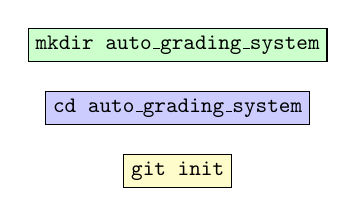
\begin{tikzpicture}[scale=0.8, transform shape]
                \node[draw, rectangle, fill=green!20] at (0,0) {\texttt{mkdir auto\_grading\_system}};
                \node[draw, rectangle, fill=blue!20] at (0,-1) {\texttt{cd auto\_grading\_system}};
                \node[draw, rectangle, fill=yellow!20] at (0,-2) {\texttt{git init}};
            \end{tikzpicture}
        \end{center}
    \end{block}

    \begin{block}{步骤2:创建虚拟环境}
        \texttt{python -m venv venv}\\
        \texttt{source venv/bin/activate}  \# Linux/Mac\\
        \texttt{venv\Scripts\activate}     \# Windows
    \end{block}

    \begin{block}{步骤3:安装依赖}
        \texttt{pip install opencv-python paddlepaddle paddleocr numpy pillow matplotlib}
    \end{block}

    \begin{block}{步骤4:创建项目结构}
        \texttt{mkdir -p modules utils data/\{input,output,templates,test\}}
    \end{block}
\end{frame}

\begin{frame}{项目目录结构}
    \begin{block}{智能阅卷系统完整结构}
        \begin{center}
            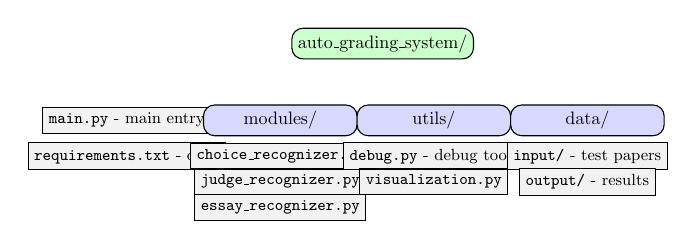
\begin{tikzpicture}[scale=0.65, transform shape,
                dir/.style={draw, rectangle, rounded corners, fill=blue!15, minimum width=3cm, minimum height=0.6cm, align=center},
                file/.style={draw, rectangle, fill=gray!10, minimum width=2.5cm, minimum height=0.5cm, align=left, font=\small},
                arrow/.style={->, thick}]

                \node[dir, fill=green!20] (root) at (5,3) {auto\_grading\_system/};

                \node[file] (main) at (0,1.5) {\texttt{main.py} - main entry};
                \node[file] (req) at (0,0.8) {\texttt{requirements.txt} - deps};

                \node[dir] (modules) at (3,1.5) {modules/};
                \node[file] (choice) at (3,0.8) {\texttt{choice\_recognizer.py}};
                \node[file] (judge) at (3,0.3) {\texttt{judge\_recognizer.py}};
                \node[file] (essay) at (3,-0.2) {\texttt{essay\_recognizer.py}};

                \node[dir] (utils) at (6,1.5) {utils/};
                \node[file] (debug) at (6,0.8) {\texttt{debug.py} - debug tools};
                \node[file] (viz) at (6,0.3) {\texttt{visualization.py}};

                \node[dir] (data) at (9,1.5) {data/};
                \node[file] (input) at (9,0.8) {\texttt{input/} - test papers};
                \node[file] (output) at (9,0.3) {\texttt{output/} - results};
            \end{tikzpicture}
        \end{center}
    \end{block}
    \begin{alertblock}{Course Materials}
        utils/debug.py and utils/visualization.py are provided (70\% framework code)
    \end{alertblock}
\end{frame}

\section{Debug Tools}

\begin{frame}{Debug Tools: save\_debug\_image}
    \textbf{Function: save\_debug\_image(image, name, output\_dir="debug")}

    \begin{block}{Purpose: Save debug images for troubleshooting}
        \begin{itemize}
            \item Creates output directory automatically
            \item Adds timestamp to filename for uniqueness
            \item Saves as PNG format
        \end{itemize}
    \end{block}

    \textbf{Usage Example:}
    \begin{center}
        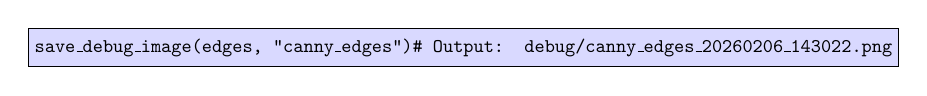
\begin{tikzpicture}[scale=0.7, transform shape]
            \node[draw, rectangle, fill=blue!15, minimum width=10cm, minimum height=0.7cm] {
                \texttt{save\_debug\_image(edges, "canny\_edges")}\\
                \texttt{\# Output: debug/canny\_edges\_20260206\_143022.png}
            };
        \end{tikzpicture}
    \end{center}
\end{frame}

\begin{frame}{Debug Tools: draw\_debug\_boxes}
    \textbf{Function: draw\_debug\_boxes(image, boxes, labels, color)}

    \begin{block}{Purpose: Visualize detection results on images}
        \begin{itemize}
            \item Draws bounding boxes on the image
            \item Optional labels for each box
            \item Customizable BGR color
        \end{itemize}
    \end{block}

    \textbf{Usage Example:}
    \begin{center}
        \begin{tikzpicture}[scale=0.7, transform shape]
            \node[draw, rectangle, fill=blue!15, minimum width=10cm, minimum height=0.7cm] {
                \texttt{debug\_img = draw\_debug\_boxes(image, boxes, ["A", "B", "C", "D"])}\\
                \texttt{save\_debug\_image(debug\_img, "detected\_boxes")}
            };
        \end{tikzpicture}
    \end{center}
\end{frame}

\begin{frame}{Debug Tools: DebugPipeline Class}
    \textbf{Class: DebugPipeline - Pipeline Step Visualization}

    \begin{block}{Key Methods:}
        \begin{itemize}
            \item \texttt{\_init\_(output\_dir="debug")} - Initialize with output directory
            \item \texttt{add\_step(name, image, info)} - Add processing step
            \item \texttt{save\_all\_steps()} - Save all step images
            \item \texttt{visualize()} - Display all steps in windows
        \end{itemize}
    \end{block}

    \textbf{Usage Example:}
    \begin{center}
        \begin{tikzpicture}[scale=0.65, transform shape]
            \node[draw, rectangle, fill=blue!15, minimum width=10cm, minimum height=1.2cm] {
                \texttt{pipeline = DebugPipeline("debug\_output")}\\
                \texttt{pipeline.add\_step("grayscale", gray)}\\
                \texttt{pipeline.add\_step("blur", blurred)}\\
                \texttt{pipeline.add\_step("edges", edges)}\\
                \texttt{pipeline.save\_all\_steps()}
            };
        \end{tikzpicture}
    \end{center}
\end{frame}

\section{Interface Design}

\begin{frame}{Module Interface Standard}
    \textbf{Recognizer Interface Definition:}

    \begin{center}
        \begin{tikzpicture}[scale=0.7, transform shape]
            \node[draw, rectangle, fill=blue!15, minimum width=10cm, minimum height=3cm, rounded corners] {
                \begin{small}
                \texttt{class BaseRecognizer:}\\
                \texttt{    """Base recognizer class"""}\\
                \texttt{    }\\
                \texttt{    def recognize(self, image, roi=None) -> RecognitionResult:}\\
                \texttt{        """Perform recognition, return result"""}\\
                \texttt{        pass}\\
                \texttt{    }\\
                \texttt{    def get\_supported\_types(self) -> List[QuestionType]:}\\
                \texttt{        """Return supported question types"""}\\
                \texttt{        pass}
                \end{small}
            };
        \end{tikzpicture}
    \end{center}

    \begin{alertblock}{Interface Contract}
        \begin{itemize}
            \item Input: image (numpy.ndarray) or ROI region
            \item Output: RecognitionResult (text, confidence, question\_type)
            \item Exception: Return result with confidence=0, no exceptions
        \end{itemize}
    \end{alertblock}
\end{frame}

\begin{frame}{RecognitionResult Data Structure}
    \textbf{Data Structure Definition:}

    \begin{center}
        \begin{tikzpicture}[scale=0.7, transform shape]
            \node[draw, rectangle, fill=green!15, minimum width=10cm, minimum height=3.5cm, rounded corners] {
                \begin{small}
                \texttt{class RecognitionResult:}\\
                \texttt{    def \_\_init\_\_(self, text, confidence, question\_type):}\\
                \texttt{        self.text = text              \# Recognized text content}\\
                \texttt{        self.confidence = confidence  \# 0.0-1.0, recognition confidence}\\
                \texttt{        self.question\_type = type    \# QuestionType enum}\\
                \texttt{        self.bounding\_box = None     \# Optional: ROI coordinates}\\
                \texttt{        self.metadata = \{\}          \# Optional: extra info}\\
                \texttt{    }\\
                \texttt{    def is\_valid(self) -> bool:}\\
                \texttt{        """Check if result is valid for grading"""}\\
                \texttt{        return self.confidence > 0.6}
                \end{small}
            };
        \end{tikzpicture}
    \end{center}
\end{frame}
              % 开发指导
%===========================================================
% 10_teamwork_extended.tex - 团队协作开发实战(扩充版)
%===========================================================

\section{AI辅助编程实战}

\begin{frame}{AI编程工具推荐}
    \textbf{课程推荐工具(按优先级):}
    \begin{columns}
        \column{0.33\textwidth}
        \begin{block}{Cursor - 首选}
            \begin{itemize}
                \item AI原生IDE
                \item Ctrl+K 原地编辑
                \item Ctrl+L 上下文对话
                \item 最适合初学者
            \end{itemize}
        \end{block}

        \column{0.33\textwidth}
        \begin{block}{Claude Code}
            \begin{itemize}
                \item 命令行AI助手
                \item 适合高级用户
                \item 强大的代码理解
            \end{itemize}
        \end{block}

        \column{0.33\textwidth}
        \begin{block}{通义灵码}
            \begin{itemize}
                \item JetBrains插件
                \item 国内访问友好
                \item 免费使用
            \end{itemize}
        \end{block}
    \end{columns}
\end{frame}

\begin{frame}{Cursor实战演示}
    \textbf{Cursor核心快捷键:}
    \begin{center}
        \begin{tikzpicture}[scale=0.9, transform shape,
            key/.style={draw, rectangle, rounded corners, fill=blue!15, minimum width=3cm, minimum height=0.6cm, align=center},
            arrow/.style={->, thick}]

            \node[key] (ctrlk) at (0,0) {\texttt{Ctrl+K} - 原地编辑代码};
            \node[key] (ctrlkdesc) at (4,0) {选中代码 → 按Ctrl+K → 输入指令};

            \node[key] (ctrlk2) at (0,-1) {\texttt{Ctrl+L} - 上下文对话};
            \node[key] (ctrldesc) at (4,-1) {询问代码逻辑、解释错误原因};

            \node[key] (ctrlk3) at (0,-2) {\texttt{Ctrl+I} - 生成新代码};
            \node[key] (ctrldesc3) at (4,-2) {描述需求 → 自动生成代码框架};
        \end{tikzpicture}
    \end{center}
\end{frame}

\begin{frame}{AI Prompt模板:RTF框架}
    \textbf{RTF框架示例 - 生成接口代码:}
    \begin{block}{Role-Task-Format}
        \begin{itemize}
            \item \textbf{Role}: 你是一个Python架构师
            \item \textbf{Task}: 设计图像预处理流水线的Filter接口
            \item \textbf{Format}: 包含类定义、方法签名、类型注解、注释
        \end{itemize}
    \end{block}

    \textbf{思维链引导示例:}
    \texttt{请一步步思考:首先确定输入输出数据结构,然后定义过滤器接口,最后实现流水线引擎}

    \textbf{少样本提示示例:}
    \texttt{请参考以下接口设计,为二值化过滤器创建类似的接口:\\
    \indent class DenoiseFilter:\\
    \indent \indent def process(self, data: ImageData) -> ImageData:}
\end{frame}

\begin{frame}{AI辅助调试三部曲}
    \textbf{遇到错误时,这样问AI:}

    \begin{enumerate}
        \item \textbf{Traceback复制}:粘贴完整的错误信息
        \item \textbf{环境说明}:Python版本、使用的库
        \item \textbf{数据贴出}:关键变量值或输入数据
    \end{enumerate}

    \begin{block}{示例Prompt}
        我遇到了这个错误:\texttt{TypeError: 'NoneType' object...}\\
        环境:Python 3.10, OpenCV 4.8\\
        代码在第56行,请帮我分析原因并修复
    \end{block}
\end{frame}

\section{调试工具函数}

\begin{frame}{调试工具函数:save\_debug\_image}
    \begin{block}{utils/debug.py}
        \lstinputlisting[
            language=Python,
            basicstyle=\ttfamily\scriptsize,
            numbers=left,
            frame=single
        ]{modules/05_development.tex}
    \end{block}
\end{frame}

\begin{frame}{调试工具函数:draw\_debug\_boxes}
    \begin{block}{绘制调试框}
        \lstinputlisting[
            language=Python,
            firstline=30,
            lastline=46,
            basicstyle=\ttfamily\scriptsize,
            numbers=left,
            frame=single
        ]{modules/05_development.tex}
    \end{block}

    \textbf{使用示例:}
    \begin{itemize}
        \item 检测到答题框后,用 \texttt{draw\_debug\_boxes} 可视化
        \item 调试时保存中间结果到 \texttt{debug/} 目录
        \item 结合 \texttt{save\_debug\_image} 记录处理步骤
    \end{itemize}
\end{frame}

\section{Git工作流实践详解}

\begin{frame}{分支策略:Git Flow详解}
    \begin{center}
        \begin{tikzpicture}[scale=0.65, transform shape,
            box/.style={draw, rectangle, rounded corners, fill=blue!15, minimum width=2.2cm, minimum height=0.6cm, align=center},
            main/.style={draw, rectangle, rounded corners, fill=red!15, minimum width=2.2cm, minimum height=0.6cm, align=center},
            develop/.style={draw, rectangle, rounded corners, fill=green!15, minimum width=2.2cm, minimum height=0.6cm, align=center}]

            % 主分支
            \node[main] (master) at (0,0) {master\\生产分支};
            \node[develop] (dev) at (0,-1.2) {develop\\开发分支};

            % 功能分支
            \node[box] (f1) at (4,-1.8) {feature/choice};
            \node[box] (f2) at (4,-2.5) {feature/judge};
            \node[box] (f3) at (4,-3.2) {feature/essay};

            % 发布分支
            \node[box, fill=yellow!15] (rel) at (8,-0.6) {release/v1.0};

            % 热修复分支
            \node[box, fill=orange!15] (hotfix) at (8,-2) {hotfix/fix};

            % 连接
            \draw[->, thick] (master) -- (dev);
            \draw[->, thick] (dev) -- (f1);
            \draw[->, thick] (dev) -- (f2);
            \draw[->, thick] (dev) -- (f3);
            \draw[->, thick] (dev) -- (rel);
            \draw[->, thick] (rel) -- (master);
            \draw[->, thick] (hotfix) -- (master);
            \draw[->, thick] (hotfix) -- (dev);
        \end{tikzpicture}
    \end{center}

    \textbf{分支说明:}
    \begin{itemize}
        \item \textbf{master}:生产分支,只接受合并,永远保持可发布状态
        \item \textbf{develop}:开发分支,功能集成分支
        \item \textbf{feature/*}:功能分支,从develop创建
        \item \textbf{release/*}:发布分支,准备上线
        \item \textbf{hotfix/*}:紧急修复,从master创建
    \end{itemize}
\end{frame}

\begin{frame}{分支命名规范}
    \begin{table}
        \centering
        \small
        \begin{tabular}{p{3cm}p{6cm}}
            \toprule
            \textbf{分支类型} & \textbf{命名规范} \\
            \midrule
            功能分支 & feature/模块-功能描述 \\
            & 如:feature/choice-recognizer \\
            \hline
            发布分支 & release/v版本号 \\
            & 如:release/v1.0.0 \\
            \hline
            修复分支 & hotfix/问题描述 \\
            & 如:hotfix/correct-bug-001 \\
            \hline
            实验分支 & dev/实验描述 \\
            & 如:dev/ocr-experiment \\
            \bottomrule
        \end{tabular}
    \end{table}

    \begin{alertblock}{命名原则}
        \begin{itemize}
            \item 使用小写字母
            \item 使用连字符(-)而非下划线
            \item 描述清晰,避免缩写
            \item 包含任务编号(如有)
        \end{itemize}
    \end{alertblock}
\end{frame}

\section{分组任务清单}

\begin{frame}{开发任务分解}
    \textbf{高优先级(P0)- 本周必须完成:}
    \begin{columns}
        \column{0.5\textwidth}
        \begin{block}{选择题识别器}
            \begin{itemize}
                \item ChoiceRecognizer类框架
                \item 填涂区域检测
                \item 像素密度统计
                \item 置信度计算
                \item 单元测试
            \end{itemize}
        \end{block}

        \column{0.5\textwidth}
        \begin{block}{判断题识别器}
            \begin{itemize}
                \item JudgeRecognizer类框架
                \item 符号轮廓提取
                \item 形状特征分析
                \item √/× 分类
                \item 单元测试
            \end{itemize}
        \end{block}
    \end{columns}

    \textbf{中优先级(P1)- 下周完成:}
    \begin{itemize}
        \item 简答题识别器(集成PaddleOCR)
        \item 评分模块
        \item 模块集成测试
    \end{itemize}

    \textbf{低优先级(P2)- 选做:}
    \begin{itemize}
        \item 性能优化
        \item 图形界面
        \item 高级功能
    \end{itemize}
\end{frame}

\begin{frame}{角色任务清单}
    \begin{table}
        \centering
        \small
        \begin{tabular}{p{2cm}p{7cm}p{3cm}}
            \toprule
            \textbf{角色} & \textbf{本周任务} & \textbf{交付物} \\
            \midrule
            组长 & 协调分工、进度跟踪、代码审查、主程序整合 & 项目周报 \\
            技术负责人 & 架构设计、技术难点攻关、代码审查 & 架构设计文档 \\
            模块开发A & 选择题识别器实现、单元测试 & choice\_recognizer.py \\
            模块开发B & 判断题识别器实现、单元测试 & judge\_recognizer.py \\
            \bottomrule
        \end{tabular}
    \end{table}

    \begin{alertblock}{协作要求}
        每日站会(15分钟):各自汇报进度、遇到的问题
    \end{alertblock}
\end{frame}

\begin{frame}{GitHub Flow简化工作流}
    \textbf{适合小团队的简化流程:}

    \begin{enumerate}
        \item \textbf{主分支保护}:master分支受保护,禁止直接推送
        \item \textbf{功能分支开发}:从master创建feature分支
        \item \textbf{提交Pull Request}:完成功能后提交PR
        \item \textbf{代码审查}:至少1人review通过
        \item \textbf{合并到主分支}:CI通过后合并
        \item \textbf{删除功能分支}:保持仓库整洁
    \end{enumerate}

    \begin{center}
        \begin{tikzpicture}[scale=0.7, transform shape,
            box/.style={draw, rectangle, rounded corners, fill=blue!15, minimum width=2.5cm, minimum height=0.7cm}]
            \node[box, fill=green!20] (master) at (0,0) {master};
            \node[box] (feature) at (3,0) {feature/xxx};
            \node[box, fill=purple!15] (pr) at (6,0) {Pull Request};
            \node[box, fill=green!20] (master2) at (9,0) {master (合并后)};

            \draw[->, thick] (master) -- (feature);
            \draw[->, thick] (feature) -- (pr);
            \draw[->, thick] (pr) -- (master2);
        \end{tikzpicture}
    \end{center}
\end{frame}

\begin{frame}{Git命令实战}
    \begin{block}{创建功能分支}
        \begin{itemize}
            \item \texttt{git checkout -b feature/choice-recognizer} - 创建并切换
            \item \texttt{git add .} - 添加修改
            \item \texttt{git commit -m "feat: 实现选择题识别器"} - 提交
        \end{itemize}
    \end{block}

    \begin{block}{推送与同步}
        \begin{itemize}
            \item \texttt{git push origin feature/choice-recognizer} - 推送到远程
            \item \texttt{git fetch origin} - 拉取远程
            \item \texttt{git rebase origin/develop} - 变基到最新
        \end{itemize}
    \end{block}
\end{frame}

\begin{frame}{代码审查流程}
    \begin{block}{代码审查(Code Review)原则}
        \begin{itemize}
            \item 所有代码必须经过review才能合并
            \item 审查关注:功能、性能、安全、风格
            \item 提出问题要具体,给出改进建议
            \item 保持尊重,对代码不对人
            \item 及时响应审查意见
        \end{itemize}
    \end{block}

    \textbf{审查清单:}
    \begin{table}
        \centering
        \small
        \begin{tabular}{p{2cm}p{8cm}}
            \toprule
            \textbf{检查项} & \textbf{内容} \\
            \midrule
            功能性 & 代码是否实现了需求?边界条件处理了吗? \\
            可读性 & 命名是否清晰?注释是否充分? \\
            可维护性 & 是否遵循设计原则?是否高内聚低耦合? \\
            性能 & 是否有明显性能问题?算法复杂度如何? \\
            安全性 & 是否有注入风险?敏感信息处理? \\
            测试 & 是否有单元测试?覆盖率高吗? \\
            \bottomrule
        \end{tabular}
    \end{table}
\end{frame}

\begin{frame}{审查评论规范}
    \begin{columns}
        \column{0.5\textwidth}
        \textbf{好的评论:}
        \begin{itemize}
            \item "这个变量名建议改为 total\_score,更清晰表达含义"
            \item "这里建议添加边界检查,防止数组越界"
            \item "这个逻辑可以用列表推导式简化,更Pythonic"
        \end{itemize}

        \column{0.5\textwidth}
        \textbf{避免的评论:}
        \begin{itemize}
            \item "这写得不对"(太笼统)
            \item "重写这段代码"(没有说明原因)
            \item "这么简单都写错"(人身攻击)
        \end{itemize}
    \end{columns}

    \begin{block}{审查评论标记}
        \begin{itemize}
            \item \textbf{[suggestion]}:建议性改进
            \item \textbf{[nitpick]}:小的格式问题
            \item \textbf{[required]}:必须修改的问题
            \item \textbf{[blocking]}:阻塞性问题
        \end{itemize}
    \end{block}
\end{frame}

\begin{frame}{冲突解决与合并}
    \begin{block}{避免冲突的最佳实践}
        \begin{itemize}
            \item 频繁提交,小步迭代
            \item 开发前先从主分支拉取最新代码
            \item 不要长时间在分支上开发
            \item 与团队成员沟通,避免同时修改同一文件
            \item 使用相同的代码格式化工具
        \end{itemize}
    \end{block}

    \textbf{解决冲突步骤:}
    \begin{center}
        \begin{tikzpicture}[scale=0.7, transform shape,
            box/.style={draw, rectangle, fill=blue!15, minimum width=5cm, minimum height=0.8cm}]
            \node[box] (step1) at (0,0) {1. git pull origin develop};
            \node[box] (step2) at (0,-1) {2. 识别冲突文件};
            \node[box] (step3) at (0,-2) {3. 编辑解决冲突};
            \node[box] (step4) at (0,-3) {4. git add <冲突文件>};
            \node[box] (step5) at (0,-4) {5. git commit};

            \draw[->, thick] (step1) -- (step2);
            \draw[->, thick] (step2) -- (step3);
            \draw[->, thick] (step3) -- (step4);
            \draw[->, thick] (step4) -- (step5);
        \end{tikzpicture}
    \end{center}
\end{frame}

\begin{frame}{版本发布管理}
    \textbf{语义化版本(Semantic Versioning):}

    \begin{center}
        \Large \textbf{MAJOR.MINOR.PATCH}
    \end{center}

    \begin{columns}
        \column{0.4\textwidth}
        \begin{itemize}
            \item \textbf{MAJOR}:不兼容的API修改
            \item \textbf{MINOR}:向下兼容的功能新增
            \item \textbf{PATCH}:向下兼容的问题修复
        \end{itemize}

        \column{0.6\textwidth}
        \begin{block}{版本示例}
            \begin{itemize}
                \item v0.1.0(内测版)
                \item v0.9.0(公测版)
                \item v1.0.0(正式版)
                \item v1.1.0(功能更新)
                \item v1.1.1(Bug修复)
            \end{itemize}
        \end{block}
    \end{columns}

    \textbf{标签操作:}
    \begin{block}{版本标签命令}
        \begin{itemize}
            \item \texttt{git tag -a v1.0.0 -m "第一个正式版本"} - 创建标签
            \item \texttt{git push origin v1.0.0} - 推送标签
            \item \texttt{git tag} - 查看标签
        \end{itemize}
    \end{block}
\end{frame}

\section{代码规范与文档}

\begin{frame}{PEP 8代码规范详解}
    \textbf{命名规范:}
    \begin{table}
        \centering
        \small
        \begin{tabular}{p{2.5cm}p{3cm}p{4.5cm}}
            \toprule
            \textbf{类型} & \textbf{规范} & \textbf{示例} \\
            \midrule
            模块/包 & 小写,短名称 & \texttt{recognition}, \texttt{utils} \\
            类 & 驼峰命名 & \texttt{ChoiceRecognizer} \\
            函数/方法 & 小写下划线 & \texttt{recognize\_choice()} \\
            变量 & 小写下划线 & \texttt{image\_data} \\
            常量 & 大写下划线 & \texttt{MAX\_IMAGE\_SIZE} \\
            私有变量 & 前导下划线 & \texttt{\_internal\_data} \\
            保护成员 & 双前导下划线 & \texttt{\_\_init\_\_} \\
            \bottomrule
        \end{tabular}
    \end{table}

    \textbf{代码布局:}
    \begin{itemize}
        \item 缩进:4个空格(禁用Tab)
        \item 行宽:最大79字符
        \item 空行:顶级函数/类间2行,方法间1行
        \item 导入:标准库→第三方→本地,每组空一行
    \end{itemize}
\end{frame}

\begin{frame}{Python代码风格检查}
    \textbf{使用工具保证代码质量:}

    \begin{columns}
        \column{0.5\textwidth}
        \textbf{black - 代码格式化}
        \begin{itemize}
            \item 强制统一代码风格
            \item 减少代码审查中的格式争论
            \item 配置简单
        \end{itemize}
        \begin{block}{安装使用}
            \begin{itemize}
                \item \texttt{pip install black}
                \item \texttt{black src/}
            \end{itemize}
        \end{block}

        \column{0.5\textwidth}
        \textbf{flake8 - 代码检查}
        \begin{itemize}
            \item 检查代码风格
            \item 发现潜在问题
        \end{itemize}
        \begin{block}{安装使用}
            \begin{itemize}
                \item \texttt{pip install flake8}
                \item \texttt{flake8 src/}
            \end{itemize}
        \end{block}
    \end{columns}
\end{frame}

\begin{frame}{类型注解与文档字符串}
    \begin{block}{类型注解示例}
        \begin{itemize}
            \item \texttt{from typing import List, Optional, Dict}
            \item \texttt{import numpy as np}
            \item 参数:\texttt{image: np.ndarray}
            \item 返回:\texttt{-> Dict[str, str]}
        \end{itemize}
    \end{block}

    \begin{block}{文档字符串规范}
        \begin{itemize}
            \item \textbf{Args}: 参数说明
            \item \textbf{Returns}: 返回值说明
            \item \textbf{Raises}: 异常说明
            \item \textbf{Example}: 使用示例
        \end{itemize}
    \end{block}
\end{frame}

\begin{frame}{接口文档生成}
    \textbf{使用工具自动生成文档:}

    \begin{columns}
        \column{0.5\textwidth}
        \textbf{Sphinx:}
        \begin{itemize}
            \item Python标准文档工具
            \item 支持reStructuredText
            \item 生成HTML/PDF/ePub
            \item 支持自动生成API文档
        \end{itemize}

        \column{0.5\textwidth}
        \textbf{MkDocs:}
        \begin{itemize}
            \item 基于Markdown
            \item 配置简单
            \item 美观的主题
            \item 适合项目文档
        \end{itemize}
    \end{columns}

        \begin{block}{pdoc文档生成}
            \begin{itemize}
                \item \texttt{pip install pdoc}
                \item \texttt{pdoc --http : mymodule} - 启动文档服务器
                \item \texttt{pdoc --html mymodule} - 生成HTML
            \end{itemize}
        \end{block}
\end{frame}

\begin{frame}{README文档规范}
    \textbf{项目README应包含:}
    \begin{table}
        \centering
        \small
        \begin{tabular}{p{3cm}p{6cm}}
            \toprule
            \textbf{章节} & \textbf{内容} \\
            \midrule
            项目名称 & 清晰的项目标题 \\
            项目简介 & 一句话描述项目目的 \\
            功能特性 & 主要功能列表 \\
            技术栈 & 使用的技术、库、版本 \\
            安装部署 & 环境要求、安装步骤 \\
            使用说明 & 快速上手示例 \\
            目录结构 & 项目文件组织 \\
            贡献指南 & 如何参与开发 \\
            许可证 & 开源协议 \\
            \bottomrule
        \end{tabular}
    \end{table}
\end{frame}

\section{团队协作实践}

\begin{frame}{任务分配与跟踪}
    \textbf{任务分解原则(WBS):}
    \begin{itemize}
        \item 每个任务可独立完成(1-3天)
        \item 任务有明确的验收标准
        \item 任务间依赖关系清晰
        \item 预留缓冲时间应对风险
    \end{itemize}

    \textbf{任务模板:}
    \begin{table}
        \centering
        \small
        \begin{tabular}{|l|l|}
            \hline
            \textbf{字段} & \textbf{示例} \\
            \hline
            任务名称 & 实现选择题识别器 \\
            任务描述 & 识别答题卡上选择题的填涂答案 \\
            验收标准 & 准确率>95\%,有单元测试 \\
            负责人 & 张三 \\
            计划工时 & 3天 \\
            截止时间 & 第10周周三 \\
            优先级 & 高 \\
            依赖任务 & 图像预处理模块 \\
            \hline
        \end{tabular}
    \end{table}
\end{frame}

\begin{frame}{每日站会与进度同步}
    \begin{block}{每日站会(Daily Stand-up)}
        \begin{itemize}
            \item 时间:固定时间,15分钟以内
            \item 形式:站立进行,保持高效
            \item 每人回答三个问题:
                \begin{enumerate}
                    \item 昨天完成了什么?
                    \item 今天计划做什么?
                    \item 有什么阻碍?
                \end{enumerate}
        \end{itemize}
    \end{block}

    \begin{columns}
        \column{0.5\textwidth}
        \textbf{进度同步工具:}
        \begin{itemize}
            \item 看板(Kanban):直观展示任务状态
            \item 燃尽图(Burndown):跟踪进度趋势
            \item 甘特图(Gantt):展示任务时间安排
        \end{itemize}

        \column{0.5\textwidth}
        \textbf{会议记录模板:}
        \begin{itemize}
            \item 日期和参会人员
            \item 各成员进度汇报
            \item 遇到的问题
            \item 解决方案
            \item 下次会议时间
        \end{itemize}
    \end{columns}
\end{frame}

\begin{frame}{问题沟通与解决}
    \textbf{问题升级路径:}

    \begin{center}
        \begin{tikzpicture}[scale=0.7, transform shape,
            box/.style={draw, rectangle, rounded corners, fill=blue!15, minimum width=4cm, minimum height=1cm, text width=3.5cm, align=center}]

            \node[box] (self) at (0,0) {1. 自主解决\\查阅文档、Google搜索};
            \node[box] (team) at (0,-1.5) {2. 团队讨论\\请教组员、技术负责人};
            \node[box] (lead) at (0,-3) {3. 组长介入\\调整方案、协调资源};
            \node[box] (teacher) at (0,-4.5) {4. 求助老师\\技术难点、方向决策};

            \draw[->, thick] (self) -- (team) node[midway, right] {30分钟};
            \draw[->, thick] (team) -- (lead) node[midway, right] {2小时};
            \draw[->, thick] (lead) -- (teacher) node[midway, right] {半天};
        \end{tikzpicture}
    \end{center}

    \begin{alertblock}{沟通原则}
        遇到问题不要憋太久,及时求助。但同时也要先自己尝试解决,带着思考去提问。
    \end{alertblock}
\end{frame}

\begin{frame}{团队协作工具链}
    \begin{center}
        \begin{tikzpicture}[scale=0.65, transform shape,
            box/.style={draw, rectangle, rounded corners, fill=blue!15, minimum width=2.5cm, minimum height=0.8cm, text width=2.3cm, align=center}]

            % 代码协作
            \node[box, fill=green!20] (git) at (0,0) {Git\\版本控制};
            \node[box, fill=green!20] (github) at (3,0) {GitHub\\代码托管};

            % 项目管理
            \node[box, fill=yellow!20] (jira) at (0,-1.2) {Jira\\任务管理};
            \node[box, fill=yellow!20] (trello) at (3,-1.2) {Trello\\看板};

            % 沟通协作
            \node[box, fill=purple!20] (slack) at (0,-2.4) {Slack\\即时通讯};
            \node[box, fill=purple!20] (confluence) at (3,-2.4) {Confluence\\文档};

            % CI/CD
            \node[box, fill=red!20] (actions) at (0,-3.6) {GitHub Actions\\CI/CD};
            \node[box, fill=red!20] (docker) at (3,-3.6) {Docker\\容器化};

            \draw[<->, thick] (git) -- (github);
            \draw[<->, thick] (jira) -- (trello);
            \draw[<->, thick] (slack) -- (confluence);
        \end{tikzpicture}
    \end{center}
\end{frame}

\begin{frame}{代码评审最佳实践}
    \textbf{评审流程:}
    \begin{center}
        \begin{tikzpicture}[scale=0.7, transform shape,
            box/.style={draw, rectangle, rounded corners, fill=blue!15, minimum width=2.5cm, minimum height=0.8cm}]
            \node[box] (create) at (0,0) {创建PR};
            \node[box] (notify) at (2.5,0) {通知Reviewer};
            \node[box] (review) at (5,0) {代码审查};
            \node[box] (revise) at (7.5,0) {修改反馈};
            \node[box, fill=green!20] (merge) at (10,0) {合并};

            \draw[->, thick] (create) -- (notify);
            \draw[->, thick] (notify) -- (review);
            \draw[->, thick] (review) -- (revise);
            \draw[->, thick] (revise) -- (merge);
        \end{tikzpicture}
    \end{center}

    \textbf{PR描述模板:}
    \begin{table}
        \centering
        \small
        \begin{tabular}{|l|p{6cm}|}
            \hline
            \textbf{字段} & \textbf{内容} \\
            \hline
            描述 & 实现选择题识别功能 \\
            关联Issue & \#123 \\
            改动内容 & 新增ChoiceRecognizer类 \\
            测试用例 & test\_choice\_recognition.py \\
            \hline
        \end{tabular}
    \end{table}
\end{frame}
        % 团队协作开发实战(扩充版)
%===========================================================
% 11_cases_extended.tex - 案例分析与互动(扩充版)
%===========================================================

\section{真实系统架构案例}

\begin{frame}{案例1:小型阅卷系统架构}
    \textbf{项目背景:}
    \begin{itemize}
        \item 用户:单个班级(约30人)
        \item 试卷量:每周100-500份
        \item 功能:选择题+判断题识别
        \item 团队:1-2人
    \end{itemize}

    \begin{center}
        \begin{tikzpicture}[scale=0.65, transform shape,
            box/.style={draw, rectangle, rounded corners, fill=blue!15, minimum width=2cm, minimum height=0.8cm, align=center}]

            % 客户端
            \node[box, fill=green!20] (web) at (0,0) {Web界面};

            % 后端
            \node[box, fill=yellow!20] (api) at (0,-1.5) {API服务器};

            % 核心模块
            \node[box] (pre) at (-3,-3) {预处理};
            \node[box] (loc) at (-1,-3) {区域定位};
            \node[box] (rec) at (1,-3) {识别};
            \node[box] (grade) at (3,-3) {评分};

            % 数据
            \node[box, fill=red!15] (file) at (0,-4.5) {文件系统};

            % 连接
            \draw[->, thick] (web) -- (api);
            \draw[->, thick] (api) -- (pre);
            \draw[->, thick] (api) -- (loc);
            \draw[->, thick] (api) -- (rec);
            \draw[->, thick] (api) -- (grade);
            \draw[->, thick] (pre) -- (file);
            \draw[->, thick] (rec) -- (file);
        \end{tikzpicture}
    \end{center}

    \textbf{架构特点:}
    \begin{itemize}
        \item 单体应用,架构简单
        \item SQLite文件存储
        \item 顺序处理,无并行
        \item 适合入门学习
    \end{itemize}
\end{frame}

\begin{frame}{案例2:中型阅卷系统架构}
    \textbf{项目背景:}
    \begin{itemize}
        \item 用户:多班级/多学校(1000+人)
        \item 试卷量:每日10000+份
        \item 功能:全题型支持
        \item 团队:5-10人
    \end{itemize}

    \begin{center}
        \begin{tikzpicture}[scale=0.65, transform shape,
            box/.style={draw, rectangle, rounded corners, minimum width=2cm, minimum height=0.8cm, align=center}]

            % 负载均衡
            \node[box, fill=purple!15] (lb) at (0,0) {负载均衡};

            % API服务
            \node[box, fill=green!20] (api1) at (-3,-1.5) {API节点1};
            \node[box, fill=green!20] (api2) at (0,-1.5) {API节点2};
            \node[box, fill=green!20] (api3) at (3,-1.5) {API节点3};

            % 处理服务
            \node[box, fill=yellow!20] (proc1) at (-4,-3) {处理服务1};
            \node[box, fill=yellow!20] (proc2) at (-1,-3) {处理服务2};
            \node[box, fill=yellow!20] (proc3) at (2,-3) {处理服务3};

            % 数据层
            \node[box, fill=red!15] (redis) at (-3,-4.5) {Redis缓存};
            \node[box, fill=red!15] (mysql) at (0,-4.5) {MySQL};
            \node[box, fill=red!15] (oss) at (3,-4.5) {对象存储};

            % 连接
            \draw[->, thick] (lb) -- (api1);
            \draw[->, thick] (lb) -- (api2);
            \draw[->, thick] (lb) -- (api3);
            \draw[->, thick] (api1) -- (proc1);
            \draw[->, thick] (api2) -- (proc2);
            \draw[->, thick] (api3) -- (proc3);
            \draw[->, thick] (proc1) -- (redis);
            \draw[->, thick] (proc2) -- (mysql);
            \draw[->, thick] (proc3) -- (oss);
        \end{tikzpicture}
    \end{center}

    \textbf{架构特点:}
    \begin{itemize}
        \item 微服务架构
        \item 水平扩展能力
        \item 数据库分库分表
        \item 缓存优化
    \end{itemize}
\end{frame}

\begin{frame}{案例3:大型企业级阅卷系统}
    \textbf{项目背景:}
    \begin{itemize}
        \item 用户:全国范围(百万用户)
        \item 试卷量:每日百万级
        \item 功能:全题型+AI辅助
        \item 团队:50+人,多团队协作
    \end{itemize}

    \begin{center}
        \begin{tikzpicture}[scale=0.55, transform shape,
            box/.style={draw, rectangle, rounded corners, minimum width=1.8cm, minimum height=0.7cm, align=center}]

            % CDN
            \node[box, fill=blue!15] (cdn) at (-5,0) {CDN};

            % API网关
            \node[box, fill=purple!15] (gateway) at (-2,0) {API网关};

            % 服务层
            \node[box, fill=green!15] (upload) at (-5,-2) {上传服务};
            \node[box, fill=green!15] (process) at (-2.5,-2) {处理服务};
            \node[box, fill=green!15] (recognize) at (0,-2) {识别服务};
            \node[box, fill=green!15] (grade) at (2.5,-2) {评分服务};
            \node[box, fill=green!15] (report) at (5,-2) {报告服务};

            % ML服务
            \node[box, fill=yellow!15] (ml1) at (0,-4) {OCR服务};
            \node[box, fill=yellow!15] (ml2) at (3,-4) {NLP服务};

            % 数据层
            \node[box, fill=red!15] (es) at (-3,-5.5) {ES搜索};
            \node[box, fill=red!15] (mysql) at (0,-5.5) {TiDB};
            \node[box, fill=red!15] (redis) at (3,-5.5) {Redis集群};

            % 连接
            \draw[->, thick] (cdn) -- (gateway);
            \draw[->, thick] (gateway) -- (upload);
            \draw[->, thick] (gateway) -- (process);
            \draw[->, thick] (gateway) -- (recognize);
            \draw[->, thick] (gateway) -- (grade);
            \draw[->, thick] (gateway) -- (report);
            \draw[->, thick] (recognize) -- (ml1);
            \draw[->, thick] (recognize) -- (ml2);
            \draw[->, thick] (upload) -- (es);
            \draw[->, thick] (grade) -- (mysql);
            \draw[->, thick] (report) -- (redis);
        \end{tikzpicture}
    \end{center}

    \textbf{架构特点:}
    \begin{itemize}
        \item 云原生架构
        \item 容器化部署(K8s)
        \item 多活容灾
        \item AI深度集成
    \end{itemize}
\end{frame}

\begin{frame}{案例对比分析}
    \begin{table}
        \centering
        \small
        \begin{tabular}{p{2cm}p{3cm}p{3cm}p{3.5cm}}
            \toprule
            \textbf{维度} & \textbf{小型} & \textbf{中型} & \textbf{大型} \\
            \midrule
            用户规模 & <1000 & 1000-10万 & 10万+ \\
            试卷量级 & 10份/天 & 1万份/天 & 100万份/天 \\
            团队规模 & 1-2人 & 5-10人 & 50+人 \\
            架构风格 & 单体分层 & 微服务 & 云原生 \\
            部署方式 & 单机部署 & 集群部署 & K8s+多活 \\
            扩展策略 & 垂直扩展 & 水平扩展 & 自动扩缩容 \\
            数据存储 & SQLite & MySQL & TiDB+ES \\
            \bottomrule
        \end{tabular}
    \end{table}

    \begin{alertblock}{选型建议}
        学生课程项目建议采用:单体分层架构 + 管道过滤器模式
        足够简单支撑当前需求,同时为未来扩展预留空间。
    \end{alertblock}
\end{frame}

\begin{frame}{架构演进路线}
    \begin{center}
        \begin{tikzpicture}[scale=0.7, transform shape,
            box/.style={draw, rectangle, rounded corners, fill=blue!15, minimum width=3cm, minimum height=0.8cm, align=center},
            arrow/.style={->, thick}]

            \node[box, fill=green!20] (phase1) at (0,0) {Phase 1: 单体\\快速上线};
            \node[box, fill=yellow!20] (phase2) at (4,0) {Phase 2: 分层\\模块解耦};
            \node[box, fill=orange!20] (phase3) at (8,0) {Phase 3: 微服务\\独立部署};
            \node[box, fill=red!20] (phase4) at (12,0) {Phase 4: 云原生\\弹性扩展};

            \draw[arrow] (phase1) -- (phase2);
            \draw[arrow] (phase2) -- (phase3);
            \draw[arrow] (phase3) -- (phase4);

            \node[box, fill=gray!15] at (6,-1.5) {
                按需演进\\
                不要过度设计
            };
        \end{tikzpicture}
    \end{center}

    \textbf{演进原则:}
    \begin{itemize}
        \item 业务驱动:扩展跟不上业务时再演进
        \item 渐进式:逐步拆分,而非一次性重写
        \item 可逆性:保持模块可独立部署能力
    \end{itemize}
\end{frame}

\section{行业最佳实践}

\begin{frame}{微服务架构最佳实践}
    \textbf{服务拆分原则:}
    \begin{enumerate}
        \item 按业务能力拆分(不是按技术)
        \item 每个服务独立数据库
        \item 服务间通过API通信
        \item 避免分布式事务
    \end{enumerate}

    \textbf{服务治理:}
    \begin{columns}
        \column{0.5\textwidth}
        \textbf{必须:}
        \begin{itemize}
            \item 服务注册发现
            \item 负载均衡
            \item 熔断降级
            \item 链路追踪
        \end{itemize}

        \column{0.5\textwidth}
        \textbf{建议:}
        \begin{itemize}
            \item API网关
            \item 配置中心
            \item 消息队列
            \item 限流
        \end{itemize}
    \end{columns}

    \begin{exampleblock}{常见问题}
        \begin{itemize}
            \item 服务拆分过细:运维复杂
            \item 服务耦合:修改影响多个服务
            \item 分布式事务:数据不一致
        \end{itemize}
    \end{exampleblock}
\end{frame}

\begin{frame}{领域驱动设计(DDD)实践}
    \textbf{核心概念:}

    \begin{columns}
        \column{0.5\textwidth}
        \textbf{战略设计:}
        \begin{itemize}
            \item 限界上下文(Bounded Context)
            \item 领域(Domain)
            \item 子域(Subdomain)
            \item 上下文映射(Context Map)
        \end{itemize}

        \column{0.5\textwidth}
        \textbf{战术设计:}
        \begin{itemize}
            \item 实体(Entity)
            \item 值对象(Value Object)
            \item 聚合(Aggregate)
            \item 领域服务(Domain Service)
        \end{itemize}
    \end{columns}

    \begin{center}
        \begin{tikzpicture}[scale=0.65, transform shape,
            box/.style={draw, rectangle, rounded corners, fill=blue!15, minimum width=2.5cm, minimum height=0.8cm}]
            \node[box] (domain) at (0,0) {阅卷领域};
            \node[box] (sub1) at (-3,-1.5) {试卷管理};
            \node[box] (sub2) at (0,-1.5) {图像处理};
            \node[box] (sub3) at (3,-1.5) {识别评分};
            \node[box] (sub4) at (0,-3) {成绩管理};

            \draw[->, thick] (sub1) -- (domain);
            \draw[->, thick] (sub2) -- (domain);
            \draw[->, thick] (sub3) -- (domain);
            \draw[->, thick] (sub4) -- (domain);
        \end{tikzpicture}
    \end{center}
\end{frame}

\begin{frame}{DevOps与CI/CD最佳实践}
    \textbf{CI/CD流水线:}

    \begin{center}
        \begin{tikzpicture}[scale=0.65, transform shape,
            box/.style={draw, rectangle, rounded corners, fill=blue!15, minimum width=1.8cm, minimum height=0.7cm}]

            \node[box, fill=green!20] (code) at (0,0) {代码提交};
            \node[box] (build) at (2.5,0) {构建};
            \node[box] (test) at (5,0) {测试};
            \node[box] (deploy) at (7.5,0) {部署};
            \node[box, fill=red!20] (prod) at (10,0) {生产环境};

            \draw[->, thick] (code) -- (build);
            \draw[->, thick] (build) -- (test);
            \draw[->, thick] (test) -- (deploy);
            \draw[->, thick] (deploy) -- (prod);
        \end{tikzpicture}
    \end{center}

    \textbf{GitHub Actions示例:}
    \begin{block}{YAML配置示例}
        \texttt{name: CI}\\
        \texttt{on: [push, pull\_request]}\\[2mm]
        \texttt{jobs:}\\
        \texttt{  build:}\\
        \texttt{    runs-on: ubuntu-latest}\\
        \texttt{    steps:}\\
        \texttt{      - uses: actions/checkout@v3}\\
        \texttt{      - name: Run tests}\\
        \texttt{        run: |}\\
        \texttt{          pip install -r requirements.txt}\\
        \texttt{          pytest}
    \end{block}
\end{frame}

\begin{frame}{测试策略最佳实践}
    \textbf{测试金字塔:}

    \begin{block}{测试分层}
        \texttt{单元测试(70\%)}\\
        \texttt{  test\_preprocessor.py, test\_recognizer.py, ...}\\[2mm]
        \texttt{集成测试(20\%)}\\
        \texttt{  test\_pipeline\_integration.py, test\_engine\_integration.py}\\[2mm]
        \texttt{端到端测试(10\%)}\\
        \texttt{  test\_full\_workflow.py, test\_api\_endpoints.py}\\[2mm]
        \texttt{快速、稳定 \hspace{3cm} 慢、复杂}
    \end{block}

    \textbf{测试原则:}
    \begin{itemize}
        \item 测试覆盖核心业务逻辑
        \item Mock外部依赖
        \item 保持测试独立
        \item 测试代码也要维护
    \end{itemize}
\end{frame}

\section{课堂互动与Quiz}

\begin{frame}{Quiz 1:架构设计判断}
    \textbf{判断正误:}

    \begin{enumerate}
        \item[1.] 微服务比单体架构更好,所以应该一开始就采用微服务。

        \item[2.] 分层架构中,上层可以跳过中间层直接调用下层。

        \item[3.] SOLID原则中的"开闭原则"指的是软件应该对扩展开放,对修改关闭。

        \item[4.] 管道-过滤器架构适合处理图像数据流。

        \item[5.] 识别器注册表可以让我们在不修改引擎代码的情况下添加新的识别算法。
    \end{enumerate}

    \begin{alertblock}{答案}
        1. 错  2. 错  3. 对  4. 对  5. 对
    \end{alertblock}
\end{frame}

\begin{frame}{Quiz 2:设计模式选择}
    \textbf{场景匹配:}

    \begin{table}
        \centering
        \small
        \begin{tabular}{p{5cm}p{5cm}}
            \toprule
            \textbf{场景} & \textbf{设计模式} \\
            \midrule
            需要在运行时切换不同的识别算法 & \\
            需要为一个类动态添加日志功能 & \\
            需要确保全局只有一个配置实例 & \\
            需要将复杂对象的构建分步骤进行 & \\
            需要在识别完成后通知评分模块 & \\
            \bottomrule
        \end{tabular}
    \end{table}

    \begin{alertblock}{参考答案}
        \begin{itemize}
            \item 运行时切换算法:策略模式
            \item 动态添加日志:装饰器模式
            \item 全局唯一实例:单例模式
            \item 分步构建:建造者模式
            \item 识别后通知:观察者模式
        \end{itemize}
    \end{alertblock}
\end{frame}

\begin{frame}{Quiz 3:架构问题诊断}
    \textbf{案例分析:}

    \begin{block}{问题描述}
        小明的智能阅卷系统运行一年后,代码变得难以维护。每次添加新题型都需要修改识别引擎的核心代码,而且经常导致原有功能出错。
    \end{block}

    \textbf{问题诊断:}
    \begin{enumerate}
        \item[1.] 识别引擎违反了哪个设计原则?
        \item[2.] 如何用设计模式解决这个问题?
        \item[3.] 如何重构代码使其更易扩展?
    \end{enumerate}

    \begin{alertblock}{参考答案}
        \begin{enumerate}
            \item 违反了开闭原则(OCP)和单一职责原则(SRP)
            \item 应用策略模式,将识别算法抽象为接口
            \item 使用工厂模式创建识别器,使用注册表管理识别器
        \end{enumerate}
    \end{alertblock}
\end{frame}

\begin{frame}{Quiz 4:场景设计}
    \textbf{设计练习:}

    \begin{block}{题目}
        请为以下场景设计解决方案:
        \begin{enumerate}
            \item[1.] 需要支持多种预处理算法(高斯滤波、中值滤波、双边滤波),用户可以选择使用哪种算法。
            \item[2.] 识别系统需要能够处理多种图片格式(PNG、JPG、TIFF)。
            \item[3.] 处理过程中需要记录每个步骤的详细信息,便于调试。
        \end{enumerate}
    \end{block}

    \textbf{设计要点:}
    \begin{center}
        \begin{tikzpicture}[scale=0.75, transform shape,
            box/.style={draw, rectangle, rounded corners, fill=blue!15, minimum width=4cm, minimum height=0.8cm}]
            \node[box] (q1) at (0,0) {1. 策略模式+工厂模式};
            \node[box] (q2) at (5,0) {2. 适配器模式};
            \node[box] (q3) at (10,0) {3. 观察者模式+日志};
        \end{tikzpicture}
    \end{center}
\end{frame}

\begin{frame}{讨论:架构决策}
    \begin{block}{讨论题目}
        在实际项目中,架构设计常常面临取舍:
        \begin{enumerate}
            \item[1.] 简单vs可扩展:对于课程项目,什么程度的架构设计是"恰到好处"?
            \item[2.] 规范vs速度:严格遵循代码规范是否会拖慢开发进度?
            \item[3.] 个人vs团队:在小团队中是否有必要使用复杂的版本控制流程?
        \end{enumerate}
    \end{block}

    \textbf{讨论要点:}
    \begin{columns}
        \column{0.5\textwidth}
        \textbf{支持严格规范:}
        \begin{itemize}
            \item 长远看节省时间
            \item 减少沟通成本
            \item 代码更易维护
        \end{itemize}

        \column{0.5\textwidth}
        \textbf{适度灵活:}
        \begin{itemize}
            \item 根据项目阶段调整
            \item 平衡成本和收益
            \item 保持核心原则
        \end{itemize}
    \end{columns}
\end{frame}

\begin{frame}{最佳实践投票(实时互动)}
    \begin{block}{手机投票说明}
        \textbf{问卷星实时投票}: 请拿出手机,扫描二维码参与投票
        \begin{itemize}
            \item 投票结果实时显示在主屏
            \item 看看其他小组的选择
            \item 准备分享你们组的决策理由
        \end{itemize}
    \end{block}

    \vspace{0.3cm}

    \textbf{投票题目:}

    \begin{columns}
        \column{0.5\textwidth}
        \begin{enumerate}
            \item[1.] 你们组打算采用什么分支策略?
                \begin{itemize}
                    \item A. Git Flow(规范)
                    \item B. GitHub Flow(简洁)
                    \item C. 主干开发(极致简化)
                \end{itemize}

            \item[2.] 识别算法通过什么方式扩展?
                \begin{itemize}
                    \item A. 配置文件(灵活)
                    \item B. 注册表(专业)
                    \item C. 硬编码(简单)
                \end{itemize}
        \end{enumerate}

        \column{0.5\textwidth}
        \begin{enumerate}
            \setcounter{enumi}{2}
            \item[3.] 代码审查的频率?
                \begin{itemize}
                    \item A. 每次PR都审查(严格)
                    \item B. 每日审查(平衡)
                    \item C. 合并前审查(宽松)
                \end{itemize}
        \end{enumerate}

        \vspace{0.5cm}

        \begin{center}
            \framebox[0.8\textwidth]{\begin{minipage}{0.75\textwidth}
                \centering
                \textbf{【扫码投票】}\\
                \vspace{0.2cm}
                \textit{(此处放置问卷星二维码)}
            \end{minipage}}
        \end{center}
    \end{columns}

    \vspace{0.3cm}

    \begin{alertblock}{投票后讨论}
        投票完成后,请选择不同选项的小组分享理由,看看能否说服对方!
    \end{alertblock}
\end{frame}

\begin{frame}{思考题}
    \begin{block}{课后思考}
        \begin{enumerate}
            \item[1.] 在识别引擎中,如果某个识别算法的准确率突然下降,如何快速定位问题?
            \item[2.] 如果要支持实时识别(边扫描边识别),流水线架构需要如何调整?
            \item[3.] 在团队协作中,如何平衡代码审查的严格程度和开发效率?
        \end{enumerate}
    \end{block}

    \begin{alertblock}{提示}
        \begin{itemize}
            \item 考虑添加监控和日志
            \item 考虑使用流式处理
            \item 考虑自动化检查工具
        \end{itemize}
    \end{alertblock}
\end{frame}
           % 案例分析与互动(扩充版)

%===========================================================
% 总结与作业
%===========================================================
%=============================================================================
% 总结与作业
%=============================================================================

\section{完整流程演示}

\begin{frame}[fragile]{阅卷系统完整流程(1/3):图像预处理}
    \textbf{目标:}将拍摄的试卷图像转换为适合处理的格式

    \begin{lstlisting}
import cv2
import numpy as np

# 1. 读取图像
img = cv2.imread('exam_paper.jpg')

# 2. 灰度化
gray = cv2.cvtColor(img, cv2.COLOR_BGR2GRAY)

# 3. 去噪
denoised = cv2.GaussianBlur(gray, (5, 5), 0)

# 4. 对比度增强
clahe = cv2.createCLAHE(clipLimit=2.0, tileGridSize=(8,8))
enhanced = clahe.apply(denoised)

# 5. 二值化
binary = cv2.adaptiveThreshold(enhanced, 255,
    cv2.ADAPTIVE_THRESH_GAUSSIAN_C,
    cv2.THRESH_BINARY, 11, 2)
    \end{lstlisting}

    \textbf{预处理步骤:}
    \begin{enumerate}
        \item \textbf{灰度化}:去除颜色信息,减少数据量
        \item \textbf{去噪}:去除扫描噪点
        \item \textbf{对比度增强}:CLAHE 自适应处理
        \item \textbf{二值化}:分离填涂和纸张
    \end{enumerate}
\end{frame}

\begin{frame}[fragile]{阅卷系统完整流程(2/3):定位答题卡}
    \textbf{目标:}在试卷中找到答题卡区域

    \begin{lstlisting}
# 1. 边缘检测
edges = cv2.Canny(binary, 50, 150)

# 2. 查找轮廓
contours, _ = cv2.findContours(edges, cv2.RETR_EXTERNAL, cv2.CHAIN_APPROX_SIMPLE)

# 3. 筛选矩形轮廓
for cnt in contours:
    peri = cv2.arcLength(cnt, True)
    approx = cv2.approxPolyDP(cnt, 0.02 * peri, True)
    if len(approx) == 4:
        x, y, w, h = cv2.boundingRect(cnt)
        answer_sheet = binary[y:y+h, x:x+w]
        break
    \end{lstlisting}
\end{frame}

\begin{frame}[fragile]{阅卷系统完整流程(3/3):识别填涂}
    \textbf{目标:}识别每个选项是否被填涂

    \begin{lstlisting}
# 定义每个选项的位置
options = [
    (50, 30, 80, 60),   # 第1题 A
    (90, 30, 120, 60),  # 第1题 B
]

results = []
for (x1, y1, x2, y2) in options:
    option = answer_sheet[y1:y2, x1:x2]
    black_ratio = np.sum(option == 0) / option.size
    is_filled = black_ratio > 0.3  # 阈值30%
    results.append(is_filled)
    \end{lstlisting}

    \textbf{识别算法优化:}
    \begin{itemize}
        \item 阈值 30\% 是经验值,可根据实际情况调整
        \item 检测是否多选,给出警告
        \item 未填涂记录,后续人工复核
    \end{itemize}
\end{frame}

% -----------------------------------------------------------------------------
% 互动测验
% -----------------------------------------------------------------------------

\section{互动测验}

\begin{frame}[fragile]{快速问答环节}
    \begin{columns}
        \column{0.5\textwidth}
        \textbf{问题1:OpenCV默认读取的彩色图像是什么顺序?}
        \begin{itemize}
            \item[A] RGB
            \item[B] \highlight{BGR}(正确)
            \item[C] HSV
            \item[D] LAB
        \end{itemize}

        \vspace{0.3cm}
        \textbf{问题2:如何判断一个图像是否读取成功?}
        \begin{itemize}
            \item[A] if img != None
            \item[B] \highlight{if img is not None}(正确)
            \item[C] if img.exists()
            \item[D] if len(img) > 0
        \end{itemize}

        \column{0.5\textwidth}
        \textbf{问题3:uint8类型的像素值范围是?}
        \begin{itemize}
            \item[A] 0-1023
            \item[B] \highlight{0-255}(正确)
            \item[C] -128-127
            \item[D] 0-65535
        \end{itemize}

        \vspace{0.3cm}
        \textbf{问题4:图像像素相加时,如何避免溢出?}
        \begin{itemize}
            \item[A] 直接相加
            \item[B] \highlight{cv2.add() 或 np.clip()}(正确)
            \item[C] 转为float后相加
            \item[D] 无需处理
        \end{itemize}
    \end{columns}

    \vspace{0.5cm}
    \begin{center}
        \highlight{正确率:\uncover<2->{\textbf{100\%} 🎉}}
    \end{center}
\end{frame}

\begin{frame}[fragile]{小测验时间(2):代码找错挑战}
    \textbf{找出以下代码中的3个错误:}

    \begin{lstlisting}
import cv2
import numpy as np

# 读取图像
img = cv2.imread('张三试卷.jpg')  # 错误1

# 亮度增加50
bright_img = img + 50  # 错误2

# 显示
plt.imshow(img)  # 错误3
plt.show()
    \end{lstlisting}

    \vspace{0.3cm}
    \begin{block}{答案揭晓}
        \begin{enumerate}
            \item \textbf{错误1:} 中文路径问题。需要使用\texttt{imread\_chinese()}函数
            \item \textbf{错误2:} 直接相加会导致溢出。应该使用\texttt{cv2.add(img, np.array([50.0]))}
            \item \textbf{错误3:} OpenCV是BGR,matplotlib是RGB。应该先转换\texttt{img = cv2.cvtColor(img, cv2.COLOR\_BGR2RGB)}
        \end{enumerate}
    \end{block}

    \vspace{0.3cm}
    \begin{center}
        \textbf{修正后的代码:}
        \begin{lstlisting}
img = imread_chinese('张三试卷.jpg')
bright_img = cv2.add(img, np.array([50.0]))
img_rgb = cv2.cvtColor(img, cv2.COLOR_BGR2RGB)
plt.imshow(img_rgb)
        \end{lstlisting}
    \end{center}
\end{frame}

% -----------------------------------------------------------------------------
% 课后作业
% -----------------------------------------------------------------------------

\section{课后作业}

\begin{frame}[fragile]{课后作业:我的第一个图像处理器}
    \begin{exampleblock}{作业要求}
        编写一个 Python 脚本,读取一张照片并生成一张包含 4 张子图的对比图:
        \begin{enumerate}
            \item 原图
            \item 灰度图
            \item 亮度增强后的图
            \item 反色后的图
        \end{enumerate}
    \end{exampleblock}
    \textbf{提交方式:} 截图 + 代码
\end{frame}

\begin{frame}{知识点网络与下周预告}
    \begin{columns}
        \column{0.6\textwidth}
        \textbf{本周核心知识点:}
        \begin{itemize}
            \item 计算机视觉基本概念
            \item 图像的数字表示(矩阵、RGB)
            \item OpenCV基础操作
            \item 图像预处理(灰度、二值化、去噪)
            \item 阅卷系统入门
        \end{itemize}

        \vspace{0.3cm}
        \textbf{下周预告(Week 2):AI辅助编程工具实战}
        \begin{itemize}
            \item \textbf{ChatGPT/Claude}:学习编程的AI助手
            \item \textbf{Prompt工程}:如何让AI帮我们写代码
            \item \textbf{实战演练}:用AI辅助实现人脸检测
        \end{itemize}

        \column{0.4\textwidth}
        \begin{block}{跨周链接}
            \begin{itemize}
                \item Week 1:图像基础 ⚙️
                \item Week 2:AI工具 🤖
                \item Week 3:图像预处理(深度) 🖼️
                \item Week 4:版面分析 📄
                \item Week 5:选择题识别 ⭕
            \end{itemize}
        \end{block}

        \vspace{0.3cm}
        \begin{alertblock}{重点提示}
        Week 2我们将学习如何用\textbf{AI工具}来加速Week 1学到的OpenCV代码开发!
        \end{alertblock}
    \end{columns}
\end{frame}

\begin{frame}{总结与问答}
    \begin{center}
        \Huge \textbf{Q \& A}
        \vspace{1cm}
        \Large 准备好进入计算机视觉的世界了吗?
    \end{center}
\end{frame}


\end{document}
